\documentclass[fleqn,10pt]{wlscirep}
%DIF LATEXDIFF DIFFERENCE FILE
%DIF DEL main_r1.tex   Wed Mar 11 20:55:32 2026
%DIF ADD main.tex      Mon Mar 16 13:40:47 2026
\usepackage[utf8]{inputenc}
\usepackage[T1]{fontenc}
\usepackage{bm}
\usepackage{caption}
\usepackage{subcaption}
% \captionsetup[subfigure]{justification=justified,singlelinecheck=false}
\usepackage{tikz}
\usepackage{newtxmath} % MER: Prettier math
\usepackage{cleveref} % MER: Allows \Cref (but use Section X.Y not Subsection X.Y)
\usepackage{booktabs} % MER: Prettier tables

\usepackage{graphicx}
\usepackage{subcaption}
\usepackage{tikz}
\usepackage{float}
\usepackage{amsmath}
\usepackage{siunitx}
\usepackage{placeins}
\usepackage{lineno}
\usetikzlibrary{quotes}
\usetikzlibrary{arrows,decorations.pathmorphing,backgrounds,positioning,fit,petri}

\graphicspath{{figures/}}

\captionsetup[subfigure]{justification=justified,singlelinecheck=false}

\title{\textcolor{black}{In-silico molecular transport via perivascular networks in the human intracranial space}}
\author[1]{Marius Causemann}
\author[1]{Miroslav Kuchta}
\author[2]{Rami Masri}
\author[1,3,*]{Marie E. Rognes }
\affil[1]{Department of Numerical Analysis and Scientific Computing, Simula Research Laboratory, Oslo, Norway}
\affil[2]{Division of Applied Mathematics, Brown University, Providence, Rhode Island, USA}
\affil[3]{K. G. Jebsen Centre for Brain Fluid Research, University of Oslo, Norway}
\affil[*]{meg@simula.no}

\newcommand{\rami}[1]{\textcolor{blue}{#1}}
\newcommand{\mer}[1]{\textcolor{magenta}{#1}}
\newcommand{\mar}[1]{\textcolor{violet}{#1}}
\newcommand{\mk}[1]{\textcolor{orange}{#1}}
\newcommand{\discuss}[1]{\textcolor{red}{#1}}
\newcommand{\fixme}[1]{\textcolor{red}{#1}}
\newcommand{\draft}[1]{\textcolor{lightgray}{#1}}

\newcommand{\R}{\mathbb{R}}
\newcommand{\foralls}{\forall \,}

\begin{abstract}
%DIF 50c50-71
%DIF <   The mechanisms of intracranial solute transport are fundamental to human brain health, with alterations often linked to disease and functional impairment, and with distinct opportunities for personalized diagnostics and treatment. However, our understanding of these mechanisms and their interplay remains incomplete, in part due to the complexity of integrating insights across scales, between species and from different modalities. Here, we combine mixed-dimensional modelling, multi-modal magnetic resonance images, and high performance computing to construct and explore a high-fidelity in-silico model of human intracranial molecular transport.  This model predicts the temporo-spatial spreading of a solute within an image-derived geometric representation of the subarachnoid space, ventricular system and brain parenchyma, including networks of surface perivascular spaces (PVSs). Our findings highlight the significant impact of cerebrospinal fluid (CSF) production and intracranial pulsatility on tracer enrichment following intrathecal tracer injection. We demonstrate that low-frequency vasomotion induces moderate CSF flow in surface PVS networks which substantially enhances tracer enrichment, and that impaired enrichment is a direct natural consequence of enlarged surface PVSs. This openly available technology platform thus provides an opportunity for integrating separate observations on diffusion in neuropil, vascular dynamics, intracranial pulsatility, CSF production, and efflux, and for exploring drug delivery and clearance in the human brain.
%DIF -------
  The mechanisms of intracranial solute transport are fundamental to %DIF > 
  human brain health, with alterations often linked to disease and %DIF > 
  functional impairment, and with distinct opportunities for %DIF > 
  personalized diagnostics and treatment. However, our understanding %DIF > 
  of these mechanisms and their interplay remains incomplete, in part %DIF > 
  due to the complexity of integrating insights across scales, between %DIF > 
  species, and from different modalities. In this work, we combine %DIF > 
  mixed-dimensional mathematical modelling, multi-modal magnetic %DIF > 
  resonance images, and high performance computing to construct a %DIF > 
  computational framework for molecular transport within the human %DIF > 
  intracranial space. The model predicts the spatiotemporal spreading %DIF > 
  of a solute within an image-derived representation of the %DIF > 
  subarachnoid space, ventricular system and brain parenchyma. A key %DIF > 
  feature is the explicit representation of surface perivascular %DIF > 
  spaces (PVSs). To illustrate applicability, we simulate a series of %DIF > 
  scenarios relating to intrathecal tracer injections, including %DIF > 
  variations in cerebrospinal fluid (CSF) production and intracranial %DIF > 
  pulsatility, perivascular fluid flow, and structural properties of %DIF > 
  the PVS. This openly available framework thus allows for evaluating %DIF > 
  the integrated effect of different transport mechanisms, bridging %DIF > 
  from the vascular mesoscale to the organ-level macroscale and across %DIF > 
  time scales of seconds to hours, in subject-specific geometries. %DIF > 
%DIF -------
\end{abstract}
%DIF PREAMBLE EXTENSION ADDED BY LATEXDIFF
%DIF UNDERLINE PREAMBLE %DIF PREAMBLE
\RequirePackage[normalem]{ulem} %DIF PREAMBLE
\RequirePackage{color}\definecolor{RED}{rgb}{1,0,0}\definecolor{BLUE}{rgb}{0,0,1} %DIF PREAMBLE
\providecommand{\DIFadd}[1]{{\protect\color{blue}\uwave{#1}}} %DIF PREAMBLE
\providecommand{\DIFdel}[1]{{\protect\color{red}\sout{#1}}} %DIF PREAMBLE
%DIF SAFE PREAMBLE %DIF PREAMBLE
\providecommand{\DIFaddbegin}{} %DIF PREAMBLE
\providecommand{\DIFaddend}{} %DIF PREAMBLE
\providecommand{\DIFdelbegin}{} %DIF PREAMBLE
\providecommand{\DIFdelend}{} %DIF PREAMBLE
\providecommand{\DIFmodbegin}{} %DIF PREAMBLE
\providecommand{\DIFmodend}{} %DIF PREAMBLE
%DIF FLOATSAFE PREAMBLE %DIF PREAMBLE
\providecommand{\DIFaddFL}[1]{\DIFadd{#1}} %DIF PREAMBLE
\providecommand{\DIFdelFL}[1]{\DIFdel{#1}} %DIF PREAMBLE
\providecommand{\DIFaddbeginFL}{} %DIF PREAMBLE
\providecommand{\DIFaddendFL}{} %DIF PREAMBLE
\providecommand{\DIFdelbeginFL}{} %DIF PREAMBLE
\providecommand{\DIFdelendFL}{} %DIF PREAMBLE
%DIF AMSMATHULEM PREAMBLE %DIF PREAMBLE
\makeatletter %DIF PREAMBLE
\let\sout@orig\sout %DIF PREAMBLE
\renewcommand{\sout}[1]{\ifmmode\text{\sout@orig{\ensuremath{#1}}}\else\sout@orig{#1}\fi} %DIF PREAMBLE
\makeatother %DIF PREAMBLE
%DIF COLORLISTINGS PREAMBLE %DIF PREAMBLE
\RequirePackage{listings} %DIF PREAMBLE
\RequirePackage{color} %DIF PREAMBLE
\lstdefinelanguage{DIFcode}{ %DIF PREAMBLE
%DIF DIFCODE_UNDERLINE %DIF PREAMBLE
  moredelim=[il][\color{red}\sout]{\%DIF\ <\ }, %DIF PREAMBLE
  moredelim=[il][\color{blue}\uwave]{\%DIF\ >\ } %DIF PREAMBLE
} %DIF PREAMBLE
\lstdefinestyle{DIFverbatimstyle}{ %DIF PREAMBLE
	language=DIFcode, %DIF PREAMBLE
	basicstyle=\ttfamily, %DIF PREAMBLE
	columns=fullflexible, %DIF PREAMBLE
	keepspaces=true %DIF PREAMBLE
} %DIF PREAMBLE
\lstnewenvironment{DIFverbatim}{\lstset{style=DIFverbatimstyle}}{} %DIF PREAMBLE
\lstnewenvironment{DIFverbatim*}{\lstset{style=DIFverbatimstyle,showspaces=true}}{} %DIF PREAMBLE
\lstset{extendedchars=\true,inputencoding=utf8}

%DIF END PREAMBLE EXTENSION ADDED BY LATEXDIFF

\begin{document}

\linenumbers

\flushbottom

\maketitle


\thispagestyle{empty}

%\mer{MER: Target length: 5000 words (Intro, Results, Discussion) plus <3000 words Methods: 700 words Introduction. 3100 words Results. 1200 words Discussion.}

\section*{Introduction}

% What is the big picture problem and why is it important? 
The mechanisms underlying molecular transport within the intracranial
space are fundamental to human brain health and
function. Neurodegenerative diseases such as Alzheimer's, Parkinson's,
and Huntington's disease are all associated with abnormal accumulation
of protein aggregates together with alterations in transport and
clearance characteristics~\cite{rasmussen2018glymphatic,
  harrison2020impaired, eide2023plasma, liu2024glymphatic}. Moreover,
sleep and conversely sleep-deprivation play a definite yet enigmatic
role in modulating molecular transport and
clearance~\cite{xie2013sleep, eide2021sleep, eide2022altered,
  miao2024brain, hauglund2025norepinephrine}. In the last decade,
established theories have been challenged by new findings on molecular
movement and exchange~\cite{iliff2012paravascular,
  ringstad2017glymphatic, louveau2017understanding,
  proulx2021cerebrospinal, bohr2022glymphatic}, including substantial
variability between individuals and between patient
cohorts~\cite{ringstad2018brain, eide2021direction, eide2021impaired,
  eide2022altered}. These observations provide distinct opportunities
(and challenges) for personalized medicine e.g.~for tailored
intrathecal delivery of chemotherapies\cite{lohela2022glymphatic} such
as methodextrate in acute lymphoblastic leukemia
patients\cite{kadan2009comparison}, and for early diagnostics of
impaired brain clearance\cite{eide2021clinical, van2024human}. In
spite of their importance, our understanding of these mechanisms is
incomplete with open challenges and significant debate -- in part
relating to the translation of knowledge between scales, species,
experimental protocols, clinical cohorts, and individuals.

Perivascular pathways along the brain surface and within the brain
parenchyma have long been hypothesized to serve a designated role in
this context~\cite{rennels1985evidence, zhang1990interrelationships,
  ichimura1991distribution, carare2008solutes, iliff2012paravascular,
  foley2012realtime, hannocks2018molecular, van2024caa}. Recently, Eide and
Ringstad~\cite{eide2024functional} and Yamamoto et
al~\cite{yamamoto2024perivascular} demonstrated that perivascular
spaces (PVSs) define preferential pathways for molecular transport in
humans, with delayed  \DIFaddbegin \DIFadd{appearance of tracer }\DIFaddend in dementia
subtypes~\cite{eide2024functional}. Perivascular flow of cerebrospinal
fluid (CSF) clearly contributes to this transport, and is inherently
associated with vascular pulsations~\cite{hadaczek2006perivascular,
  iliff2013cerebral, bedussi2018paravascular, mestre2018flow,
  boster2023artificial, hirschler2024region}. Fluid mechanics
considerations point at intracranial pressure differences and shorter
wavelength vascular wall pulsations as drivers of directional net flow
and convection in the PVS~\cite{bilston2003arterial, rey2018pulsatile,
  daversin2020mechanisms, kedarasetti2020functional,
  gjerde2023directional, nozaleda2024arterial}, while longer waves
such as the pulse wave primarily contribute to oscillatory flow and
dispersion~\cite{asgari2016glymphatic, sharp2019dispersion, thomas2019fluid,
  kedarasetti2020arterial, troyetsky2021dispersion, 
  martinac2021phase}. In the bigger picture, CSF is produced by the
choroid plexus~\cite{damkier2013cerebrospinal,
  steffensen2018cotransporter, liu2020direct}, pulsates through the
ventricular system, cisterns, and subarachnoid space (SAS) in
association with cardiac, respiratory, and neural
waves~\cite{greitz1993pulsatile, wagshul2011pulsating,
  sweetman2011cerebrospinal, fultz2019coupled, vinje2019respiratory,
  eide2021direction, causemann2022human, williams2023neural,
  zimmermann2023total}, and drains via the dural sinuses, meningeal
lymphatics, cranial nerves, or other efflux
pathways~\cite{proulx2021cerebrospinal}. However, how these
physiological factors and physical mechanisms integrate to enhance or
impair human intracranial molecular transport over larger spatial
scales and longer time scales remain unknown. A related key question
is to what extent surface PVSs are separated from the SAS by
structural barriers~\cite{zhang1990interrelationships,
  weller2005microscopic, bedussi2017paravascular,
  pizzo2018intrathecal, mestre2022periarteriolar,
  mollgard2023mesothelium, smets2024perivascular, eide2024functional},
and in turn to what extent such structural compartmentalization is a
prerequisite for effective perivascular transport.

%DIF <  What are our research questions and how do we answer them
%DIF >  Main contribution
In this study, by leveraging geometric model reduction and
mixed-dimensional modelling~\cite{masri2024modelling}, structural
magnetic resonance (MR) images~\cite{hodneland2019new}, and high
performance computing, we introduce an  \DIFaddbegin \DIFadd{integrative computational
framework for modelling }\DIFaddend intracranial molecular transport. Focusing on
the interplay between perivascular pathways, pulsatility and CSF flow
dynamics,  \DIFaddbegin \DIFadd{our models predict the }\DIFaddend temporal evolution and spatial
distribution of a solute concentration within a detailed geometric
representation of the human SAS and ventricular system, in networks of
surface PVSs (i.e.~those surrounding arteries and veins in the SAS),
and in the brain parenchyma. In terms of transport dynamics, we
account for heterogeneous diffusion, dispersive mixing induced by
cardiac and respiratory pulsatility in the CSF spaces , convective
fluid flow driven by CSF production \DIFaddbegin \DIFadd{in the CSF spaces }\DIFaddend and peristaltic
pumping \DIFaddbegin \DIFadd{in the PVSs}\DIFaddend , as well as solute exchange and clearance across
semi-permeable membranes.  \DIFaddbegin \DIFadd{Preliminary comparisons indicate that the
in-silico model predictions align well with the range of tracer distribution
patterns reported in contrast-enhanced }\DIFaddend MRI
studies~\cite{ringstad2017glymphatic, ringstad2018brain,
  watts2019measuring, eide2024functional} \DIFaddbegin \DIFadd{.
}

\DIFadd{Our key contribution is thus an }\DIFaddend in-silico  \DIFaddbegin \DIFadd{modelling framework that
allows for evaluating the integrated effect of different proposed
transport mechanisms, bridging from the vascular mesoscale to the
organ-level macroscale and across time scales of seconds to days, in
subject-specific geometries. This concept provides a missing link to
bridge mesoscale phenomena -- such as perivascular pulsations occuring
every few seconds -- with macroscale observations of tissue-level
tracer distribution over hours to days. We illustrate the range of
this computational framework via a series of model scenarios motivated
by key }\DIFaddend questions relating to molecular movement within the human brain
environment \DIFaddbegin \DIFadd{. In particular, we explore how }\DIFaddend the balance between CSF
production and intracranial pulsatility  \DIFaddbegin \DIFadd{can shape }\DIFaddend large-scale features
of  \DIFaddbegin \DIFadd{the tracer distribution. We examine how perivascular }\DIFaddend fluid flow
induced by \DIFaddbegin \DIFadd{cardiac pulsations or }\DIFaddend low-frequency vasomotion  \DIFaddbegin \DIFadd{can be
expected to impact tracer arrival times within the surrounding CSF
spaces and parenchyma. Finally, we study how changes in structural
properties, such as }\DIFaddend the absence of a structural compartmentalization
of the PVS  \DIFaddbegin \DIFadd{or enlarged PVSs, can impact perivascular transport }\DIFaddend and
 \DIFaddbegin \DIFadd{intracranial tracer spread. The openly available technology
platform\mbox{%DIFAUXCMD
\cite{ZENODO} }\hskip0pt%DIFAUXCMD
allows for transferring, integrating, and
examining }\DIFaddend insights from clinical, experimental, and theoretical
studies, and  \DIFaddbegin \DIFadd{provides a starting-point }\DIFaddend for future in-silico studies of
 \DIFaddbegin \DIFadd{brain solute transport}\DIFaddend .

\section*{Results}

%DIF > \fixme{We present a computational framework first, and then demonstrate it by simulating a contrast-enhanced MRI protocol, including a series of model variations.}
\DIFaddbegin 

\DIFaddend \subsection*{ \DIFaddbegin \DIFadd{An integrative computational framework for }\DIFaddend intracranial \DIFaddbegin \DIFadd{solute }\DIFaddend transport  \DIFaddbegin \DIFadd{informed by multi-modal MRI}\DIFaddend }
\DIFaddbegin 

\DIFaddend \begin{figure}
    \centering
     \DIFaddbeginFL \vspace{40em}
    %DIF > 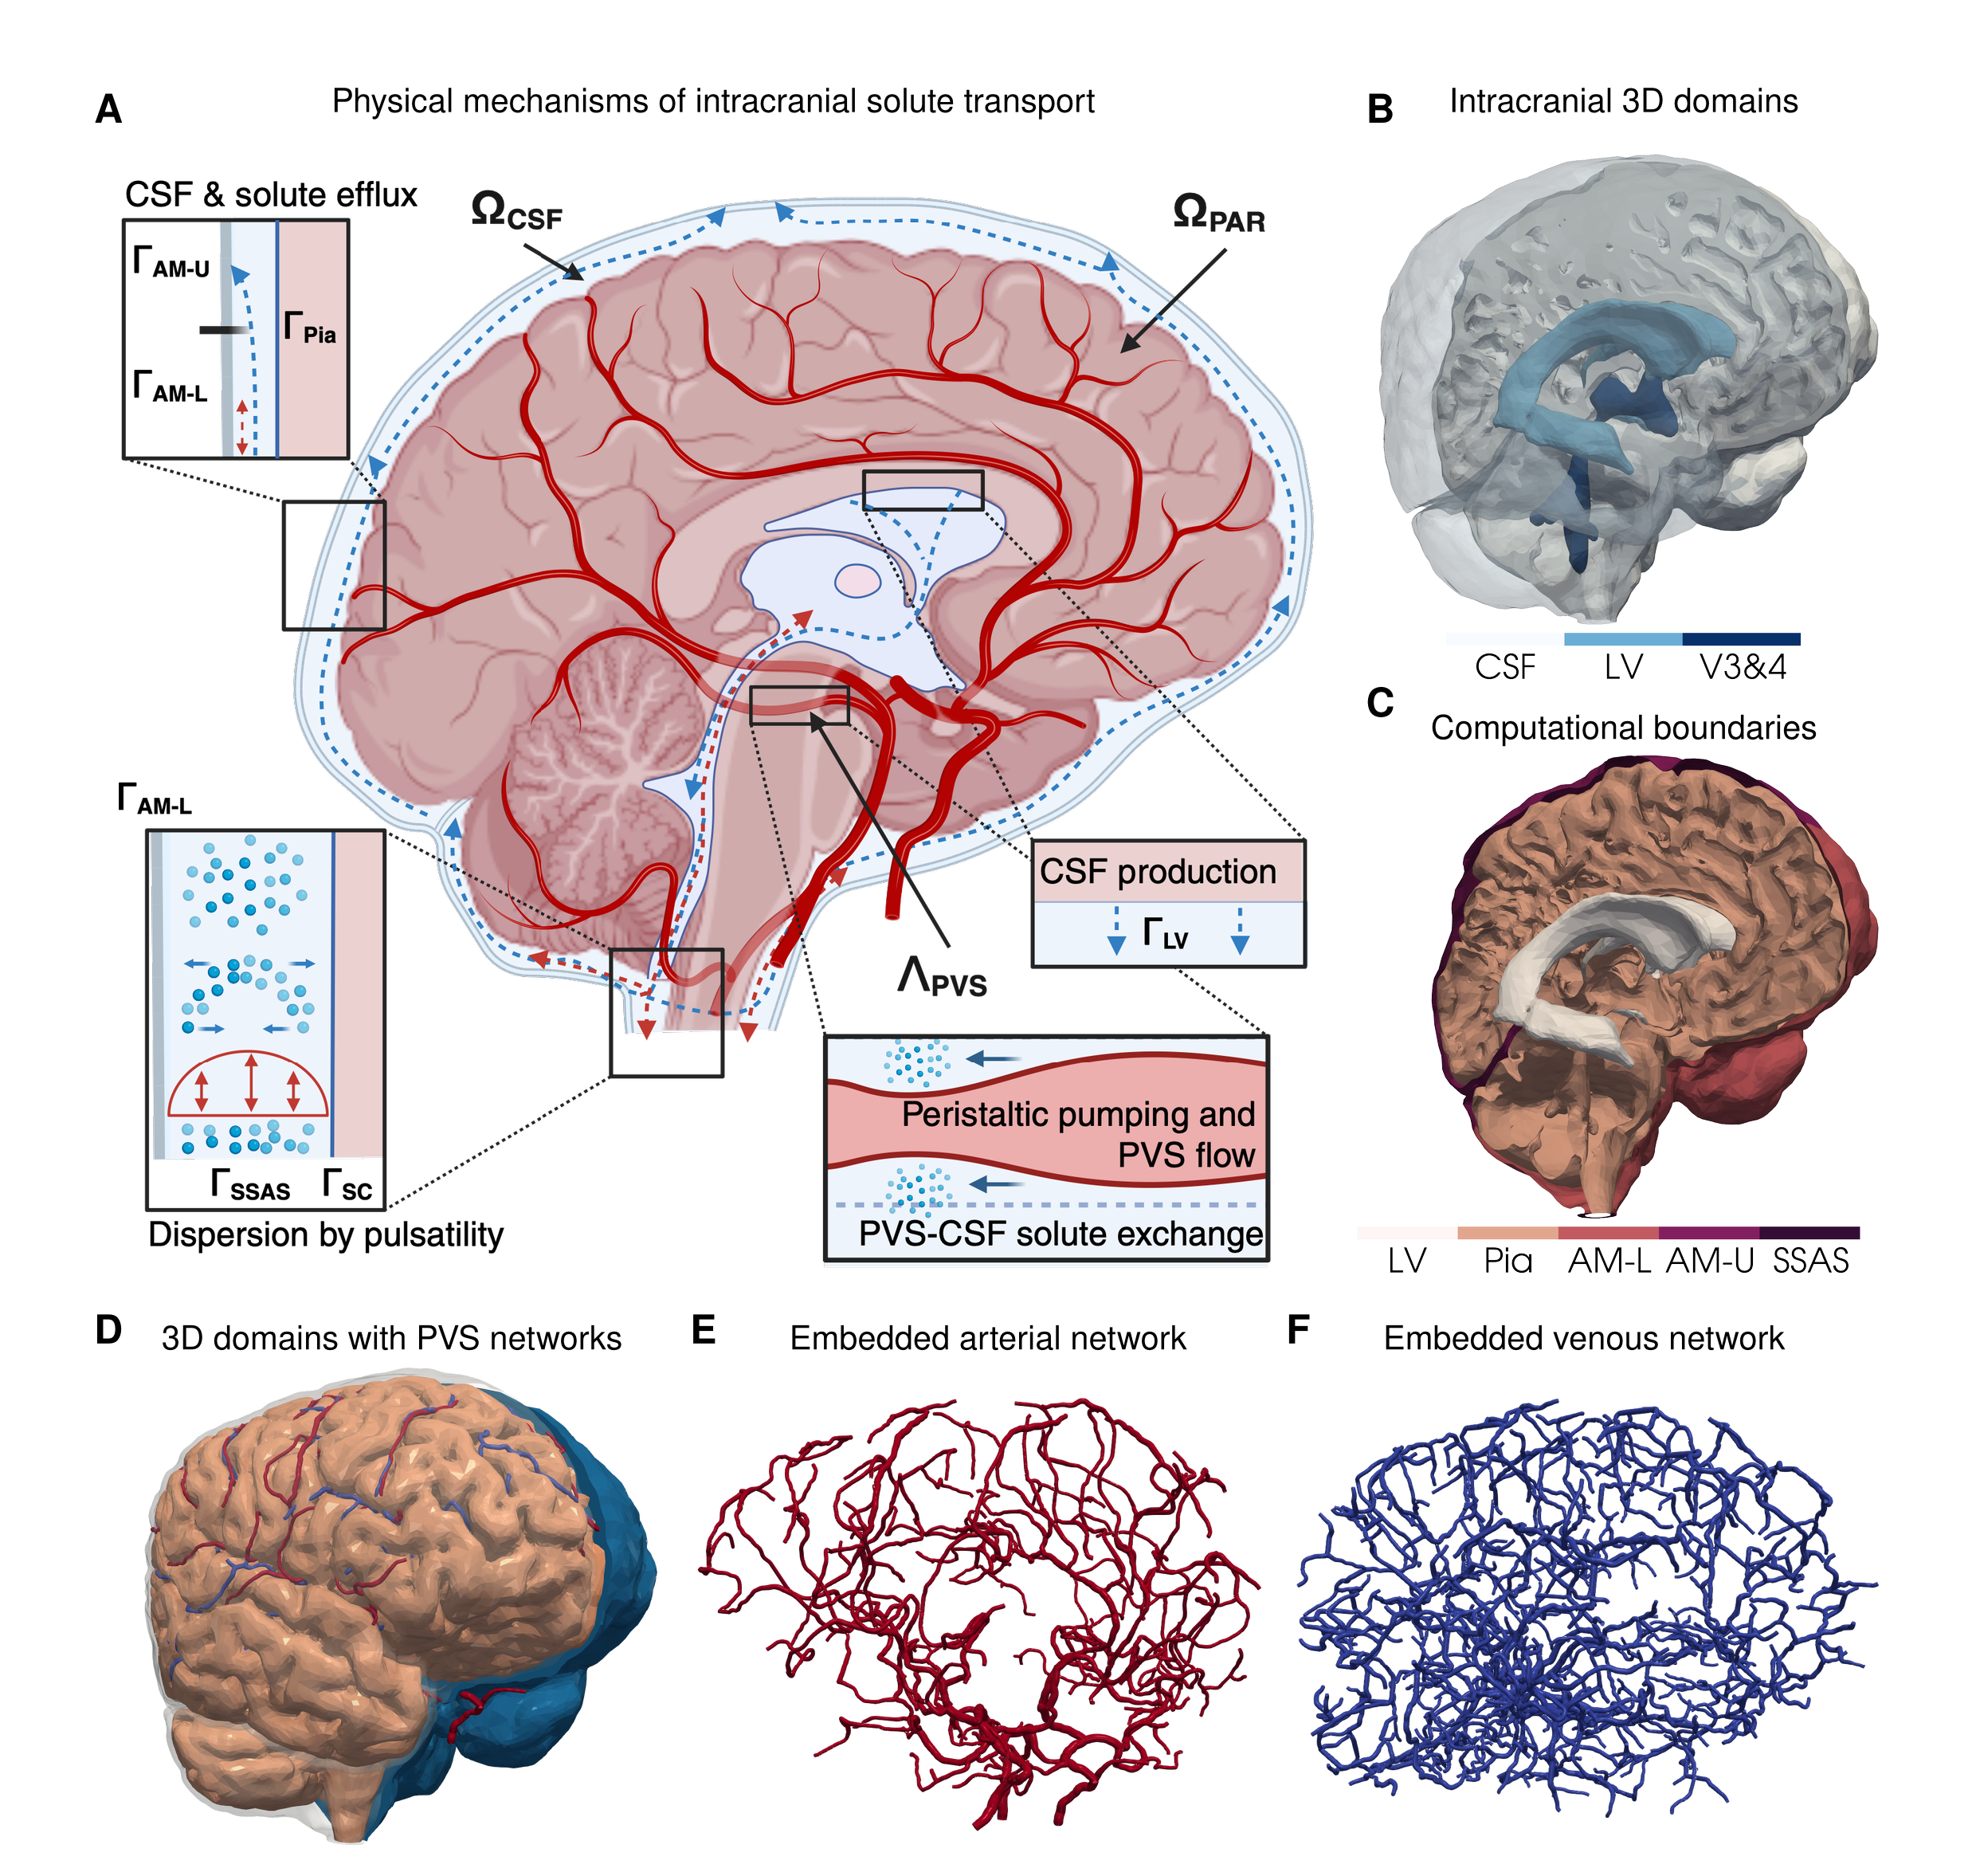
\includegraphics[width=1\textwidth]{figures/figure1.png}
     \DIFaddendFL \caption{
      \DIFaddbeginFL \textbf{\DIFaddFL{An integrative computational framework for intracranial solute transport.}}\DIFaddendFL }
     \label{fig:results1}
\end{figure}
\DIFaddbegin 

\begin{figure}
    \centering
    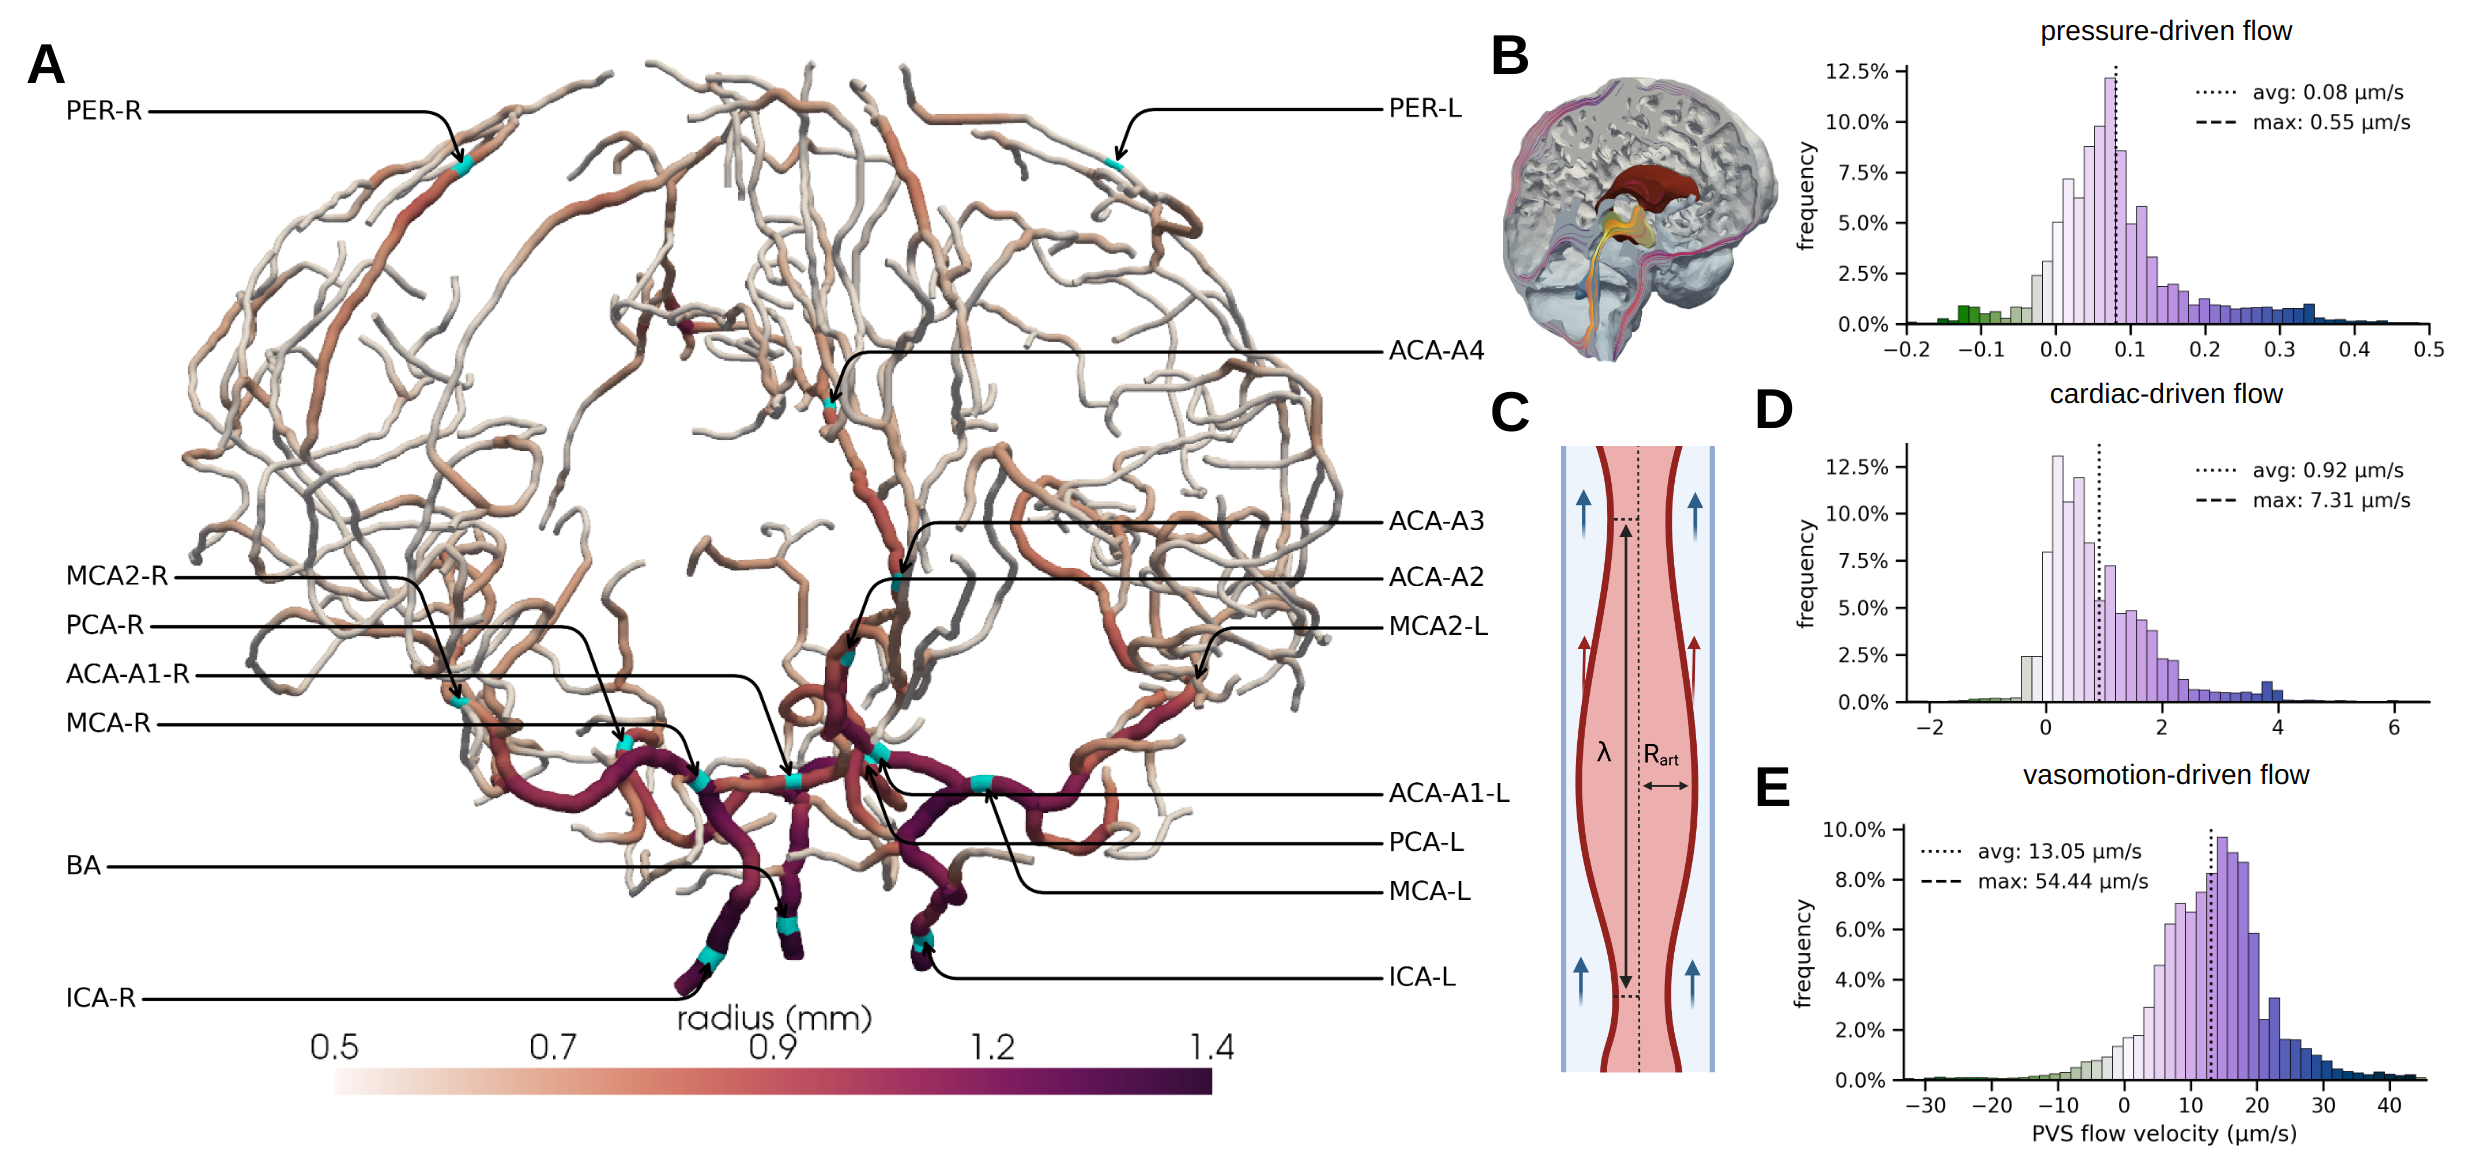
\includegraphics[width=0.95\textwidth]{figures/figure3a.png}
    \caption{\DIFaddFL{\fixme{\textbf{A static pressure gradient and peristaltic pumping are potential drivers of perivascular flow.}}
    A) Surface arterial network colored by arterial radius with vessel locations labeled;
    B) Net PVS flow induced by CSF production alone (see also~\mbox{%DIFAUXCMD
\Cref{fig:csf}}\hskip0pt%DIFAUXCMD
D).
    Histograms show the relative frequencies of local periarterial velocities. Positive values indicate antegrade PVS flow, while negative values indicate retrograde PVS flow;
    C) Illustration of the concept of peristaltic pumping;
    D) histograms of estimated net PVS flow induced by pulse wave or vasomotion peristaltic pumping;
    E) Estimated net PVS flow induced by pulse wave peristaltic pumping alone.
    F) Estimated net PVS flow induced by vasomotion/slow wave peristaltic pumping alone.}}
    \label{fig:pvs}
\end{figure}

\DIFaddend Using previously published multi-modal magnetic resonance imaging
(MRI) data~\cite{hodneland2019new, deistung2009tof,
  schweser2012quantitative, reichenbach2012future,
  deistung2017overview}, we construct a multiscale computational
representation of the human intracranial compartments consisting of
the CSF spaces and brain parenchyma as three-dimensional (3D) domains
and with the PVSs surrounding major surface arteries and veins as
embedded networks of topologically one-dimensional (1D) curves
( \DIFaddbegin \DIFadd{\fixme{\Cref{fig:results1}}). As the drivers and modes of
intracranial transport are under substantial uncertainty and
debate\mbox{%DIFAUXCMD
\cite{smith2019going, proulx2021cerebrospinal,
  bohr2022glymphatic, hladky2022glymphatic, betsholtz2024advances,
  kipnis2025resolving}}\hskip0pt%DIFAUXCMD
, our target is to introduce a computational
framework that allows for integrating and evaluating different
transport mechanisms, and in particular perivascular pathways, in
subject-specific geometries.
}

\DIFadd{To this end, we introduce the following modelling choices
(\fixme{\Cref{fig:results1}}, see also Methods). We define
\fixme{three} solute concentration fields, each }\DIFaddend varying in space and
time, \DIFaddbegin \DIFadd{one }\DIFaddend in the 3D domains and  \DIFaddbegin \DIFadd{one in each of }\DIFaddend the PVS networks, and
assume that the solute can cross between  \DIFaddbegin \DIFadd{the 3D and 1D domains via
}\DIFaddend semi-permeable membranes.  \DIFaddbegin \DIFadd{We }\DIFaddend assume that the solute will  diffuse
within all compartments, with diffusivity depending on the effective
properties of the relevant medium\cite{sykova2008diffusion} \DIFaddbegin \DIFadd{. We assume
that flow in the CSF spaces will substantially affect solute
transport, and we account for two main mechanisms
(\fixme{\Cref{fig:results1}}): (i) convection via }\DIFaddend a (small) net flow
of CSF resulting from production in the choroid plexus with CSF efflux
across the upper convexity\cite{hornkjol2022csf} \DIFaddbegin \DIFadd{, and (ii) dispersive
effects resulting from the pulsatile flow of
CSF~\mbox{%DIFAUXCMD
\cite{sweetman2011cerebrospinal, vinje2019respiratory,
  ray2021quantitative}}\hskip0pt%DIFAUXCMD
. In the }\DIFaddend surface periarterial spaces \DIFaddbegin \DIFadd{, we account
for convection via net fluid flow induced by peristaltic
pumping~\mbox{%DIFAUXCMD
\cite{mestre2018flow, gjerde2023directional}
}\hskip0pt%DIFAUXCMD
(\fixme{\Cref{fig:pvs}}).  Specifically, we introduce the
geometrically-reduced representation of the PVSs to bridge spatial
scales, and model pulsatility via dispersion in the CSF and
time-averaged flow in the PVS to bridge temporal
scales. Mathematically, the solute transport }\DIFaddend model is represented by a
mixed-dimensional system of coupled time-dependent partial
differential equations\cite{masri2024modelling}, which we solve
numerically with high accuracy using a mass-conserving finite element
scheme \DIFaddbegin \DIFadd{. The complete computational framework is implemented in }\DIFaddend the
FEniCS finite element software \cite{alnaes2015fenics,
  kuchta2020assembly} \DIFaddbegin \DIFadd{, and all associated software is }\DIFaddend all openly
available~\cite{ZENODO}.


 \DIFaddbegin \DIFadd{To inform the convective velocity fields and dispersion factors
entering as coefficients in the transport equations, we define
auxiliary flow models in the CSF spaces and PVSs
(\fixme{\Cref{fig:results1}}, \fixme{\Cref{fig:pvs}}). Beginning with
flow field driven by CSF production, we impose a CSF inflow of $400$
mL/day into the lateral ventricles (\fixme{\Cref{fig:results1}}),
yielding a maximum flow velocity of $1.85\,$mm/s (in the aqueduct) and
a mean velocity in the SAS of $2.6$ }\textmu \DIFadd{m/s
(\fixme{\Cref{fig:results1}}). To estimate the dispersive effect of
pulsatile CSF flow, we employ the theory of shear-augmented dispersion
together with computational fluid dynamics to determine
spatially-varying dispersion factors $R_c, R_r$ enhancing the
effective solute diffusivity in the CSF spaces by $R = R_c + R_r$ (see
Methods). Assuming a cardiac frequency of $1\,$Hz, we infer that the
cardiac-induced pulsatile CSF flow increases the effective diffusion
by more than two orders of magnitude in the aqueduct and near the
cisterna magna, but has little effect ($R_c < 1$) in most of the SAS
(\fixme{\Cref{fig:results1}}). The dispersive effect from respiration
reaches a factor of up to 320 due the lower respiratory frequency of
$0.25\,$Hz (\fixme{\Cref{fig:results1}}).
}

\DIFadd{Traveling waves of arterial wall motion (\fixme{\Cref{fig:pvs}C}),
such as the pulse wave or other
vasomotion~\mbox{%DIFAUXCMD
\cite{vanveluw2020vasomotion, munting2023spontaneous,
  bojarskaite2023sleep, broggini2024long,hauglund2025norepinephrine}}\hskip0pt%DIFAUXCMD
,
can induce net directional flow in the
PVS~\mbox{%DIFAUXCMD
\cite{kedarasetti2020arterial, kedarasetti2020functional,
  coenen2021lubrication, gjerde2023directional, nozaleda2024arterial}
}\hskip0pt%DIFAUXCMD
-- of magnitude and direction depending on the amplitude, frequency,
and length of the waves and the characteristics of the perivascular
network~\mbox{%DIFAUXCMD
\cite{gjerde2023directional}}\hskip0pt%DIFAUXCMD
. Our periarterial network extends
from the internal carotid arteries and basilar artery through up to 18
bifurcations to reach upstream network ends located within the SAS or
up to 6 mm inside the parenchyma and includes major surface arteries
of radius 0.5--1.4 mm (\mbox{%DIFAUXCMD
\Cref{fig:pvs}}\hskip0pt%DIFAUXCMD
). Due to imaging limitations,
the network primarily covers the supratentorial regions, with the
lowest network point located approximately $4\,$cm above the
craniocervical junction. Applying a semi-analytic model of the net
flow induced by peristalsis in this periarterial
network~\mbox{%DIFAUXCMD
\cite{gjerde2023directional} }\hskip0pt%DIFAUXCMD
(see Methods), we estimate that
the cardiac pulse wave alone, traveling at a frequency of 1 Hz with a
wavelength of 2.0 m and a 1\% wall displacement~\mbox{%DIFAUXCMD
\cite{jung2021novel}}\hskip0pt%DIFAUXCMD
,
will induce mainly antegrade perivascular flow with an average net velocity of
0.92 }\textmu \DIFadd{m/s while reaching up to 7.31 }\textmu \DIFadd{m/s near larger,
ventral vessels such as the MCA (\mbox{%DIFAUXCMD
\Cref{fig:pvs}}\hskip0pt%DIFAUXCMD
D,E), and a total flow
through the periarterial network of $\fixme{10.5}$ mL/day. The same
theory predicts that strong ultraslow vasomotions, if traveling
antegrade at 0.1Hz with a wavelength of 0.02 m and a 10\%
displacement~\mbox{%DIFAUXCMD
\cite{broggini2024long}}\hskip0pt%DIFAUXCMD
, will induce both retrograde and
antegrade net perivascular flow with an average velocity of 13.05 }\textmu \DIFadd{m/s
and maximum velocity 54.44 }\textmu \DIFadd{m/s, and a total flow of
$\fixme{X}$ mL/day (\mbox{%DIFAUXCMD
\Cref{fig:pvs}}\hskip0pt%DIFAUXCMD
D,F). \fixme{Add 1-2 sentence about decoupled flow modelling here.}
}


\subsection*{\DIFadd{In-silico predictions of tracer distribution after intrathecal injection in cardiac and respiratory flow regimes}}

\DIFadd{Intrathecal administration of gadolinium-based contrast agents in
combination with MR imaging has emerged as a key technique to study
solute distribution and clearance in the human
brain~\mbox{%DIFAUXCMD
\cite{ringstad2017glymphatic, ringstad2018brain,
  eide2024functional, van2024human, kipnis2025resolving}}\hskip0pt%DIFAUXCMD
. To simulate
such a contrast-enhanced }\DIFaddend MRI protocol~\cite{ringstad2017glymphatic,
  ringstad2018brain,
  eide2024functional}( \DIFaddbegin \DIFadd{\fixme{\Cref{fig:intrathecal}C}}\DIFaddend ), we  \DIFaddbegin \DIFadd{now apply
our computational framework to }\DIFaddend predict the spreading of $0.5$ mmol
intrathecally injected Gadobutrol after its appearance at the
craniocervical junction, represented by tracer inflow across the
spinal SAS boundary over the first two hours
( \DIFaddbegin \DIFadd{\fixme{\Cref{fig:intrathecal}D--E}). To begin with, we consider a
reasonably conservative set of flow patterns: modelling the dispersive
effects of pulsatile CSF flow induced by the cardiac and respiratory
cycles~\mbox{%DIFAUXCMD
\cite{sweetman2011cerebrospinal, vinje2019respiratory} }\hskip0pt%DIFAUXCMD
and the
periarterial net flow induced by cardiac pulse waves
alone~\mbox{%DIFAUXCMD
\cite{mestre2018flow, gjerde2023directional}}\hskip0pt%DIFAUXCMD
.
}

\DIFaddend After one hour, the in-silico tracer moves upwards in the SAS
frontally of the brainstem, and quickly reaches the supratentorial
regions. Here, it spreads both posterior through the quadrigeminal
cistern and the longitudinal fissure, and anteriorly through the outer
SAS, reaching the top of the cerebral cortex after around 12
hours. After 24 hours, the tracer covers most of the brain surface
(with the exception of some posterior regions) and has penetrated
substantially into the parenchymal tissue. This pattern is reflected
in the mean tracer concentrations in each compartment, where the CSF
space reaches its peak of $1.4\,$mmol/l after 2 hours, followed by the
arterial PVS concentration peak ($2.9\,$mmol/l after 4 hours)
( \DIFaddbegin \DIFadd{\fixme{\Cref{fig:intrathecal}F}}\DIFaddend ). While the mean concentrations in these
compartments drop soon after peaking, the  \DIFaddbegin \DIFadd{concentration in the
parenchyma increases more slowly }\DIFaddend over the first 24 hours, with a final
value of $0.3$ mmol/l. Overall, about 40\% of the total amount of
tracer remains in the cranium 24 hours post-injection \DIFaddbegin \DIFadd{in this baseline
simulation}\DIFaddend , with the largest share in the CSF (53\%), followed by the
parenchyma (35\%), the venous PVS (8\%) and the arterial PVS (5\%)
( \DIFaddbegin \DIFadd{\fixme{\Cref{fig:intrathecal}G}}\DIFaddend ).

 \begin{figure}
    %DIF < [h!]
\centering
     \DIFaddbeginFL 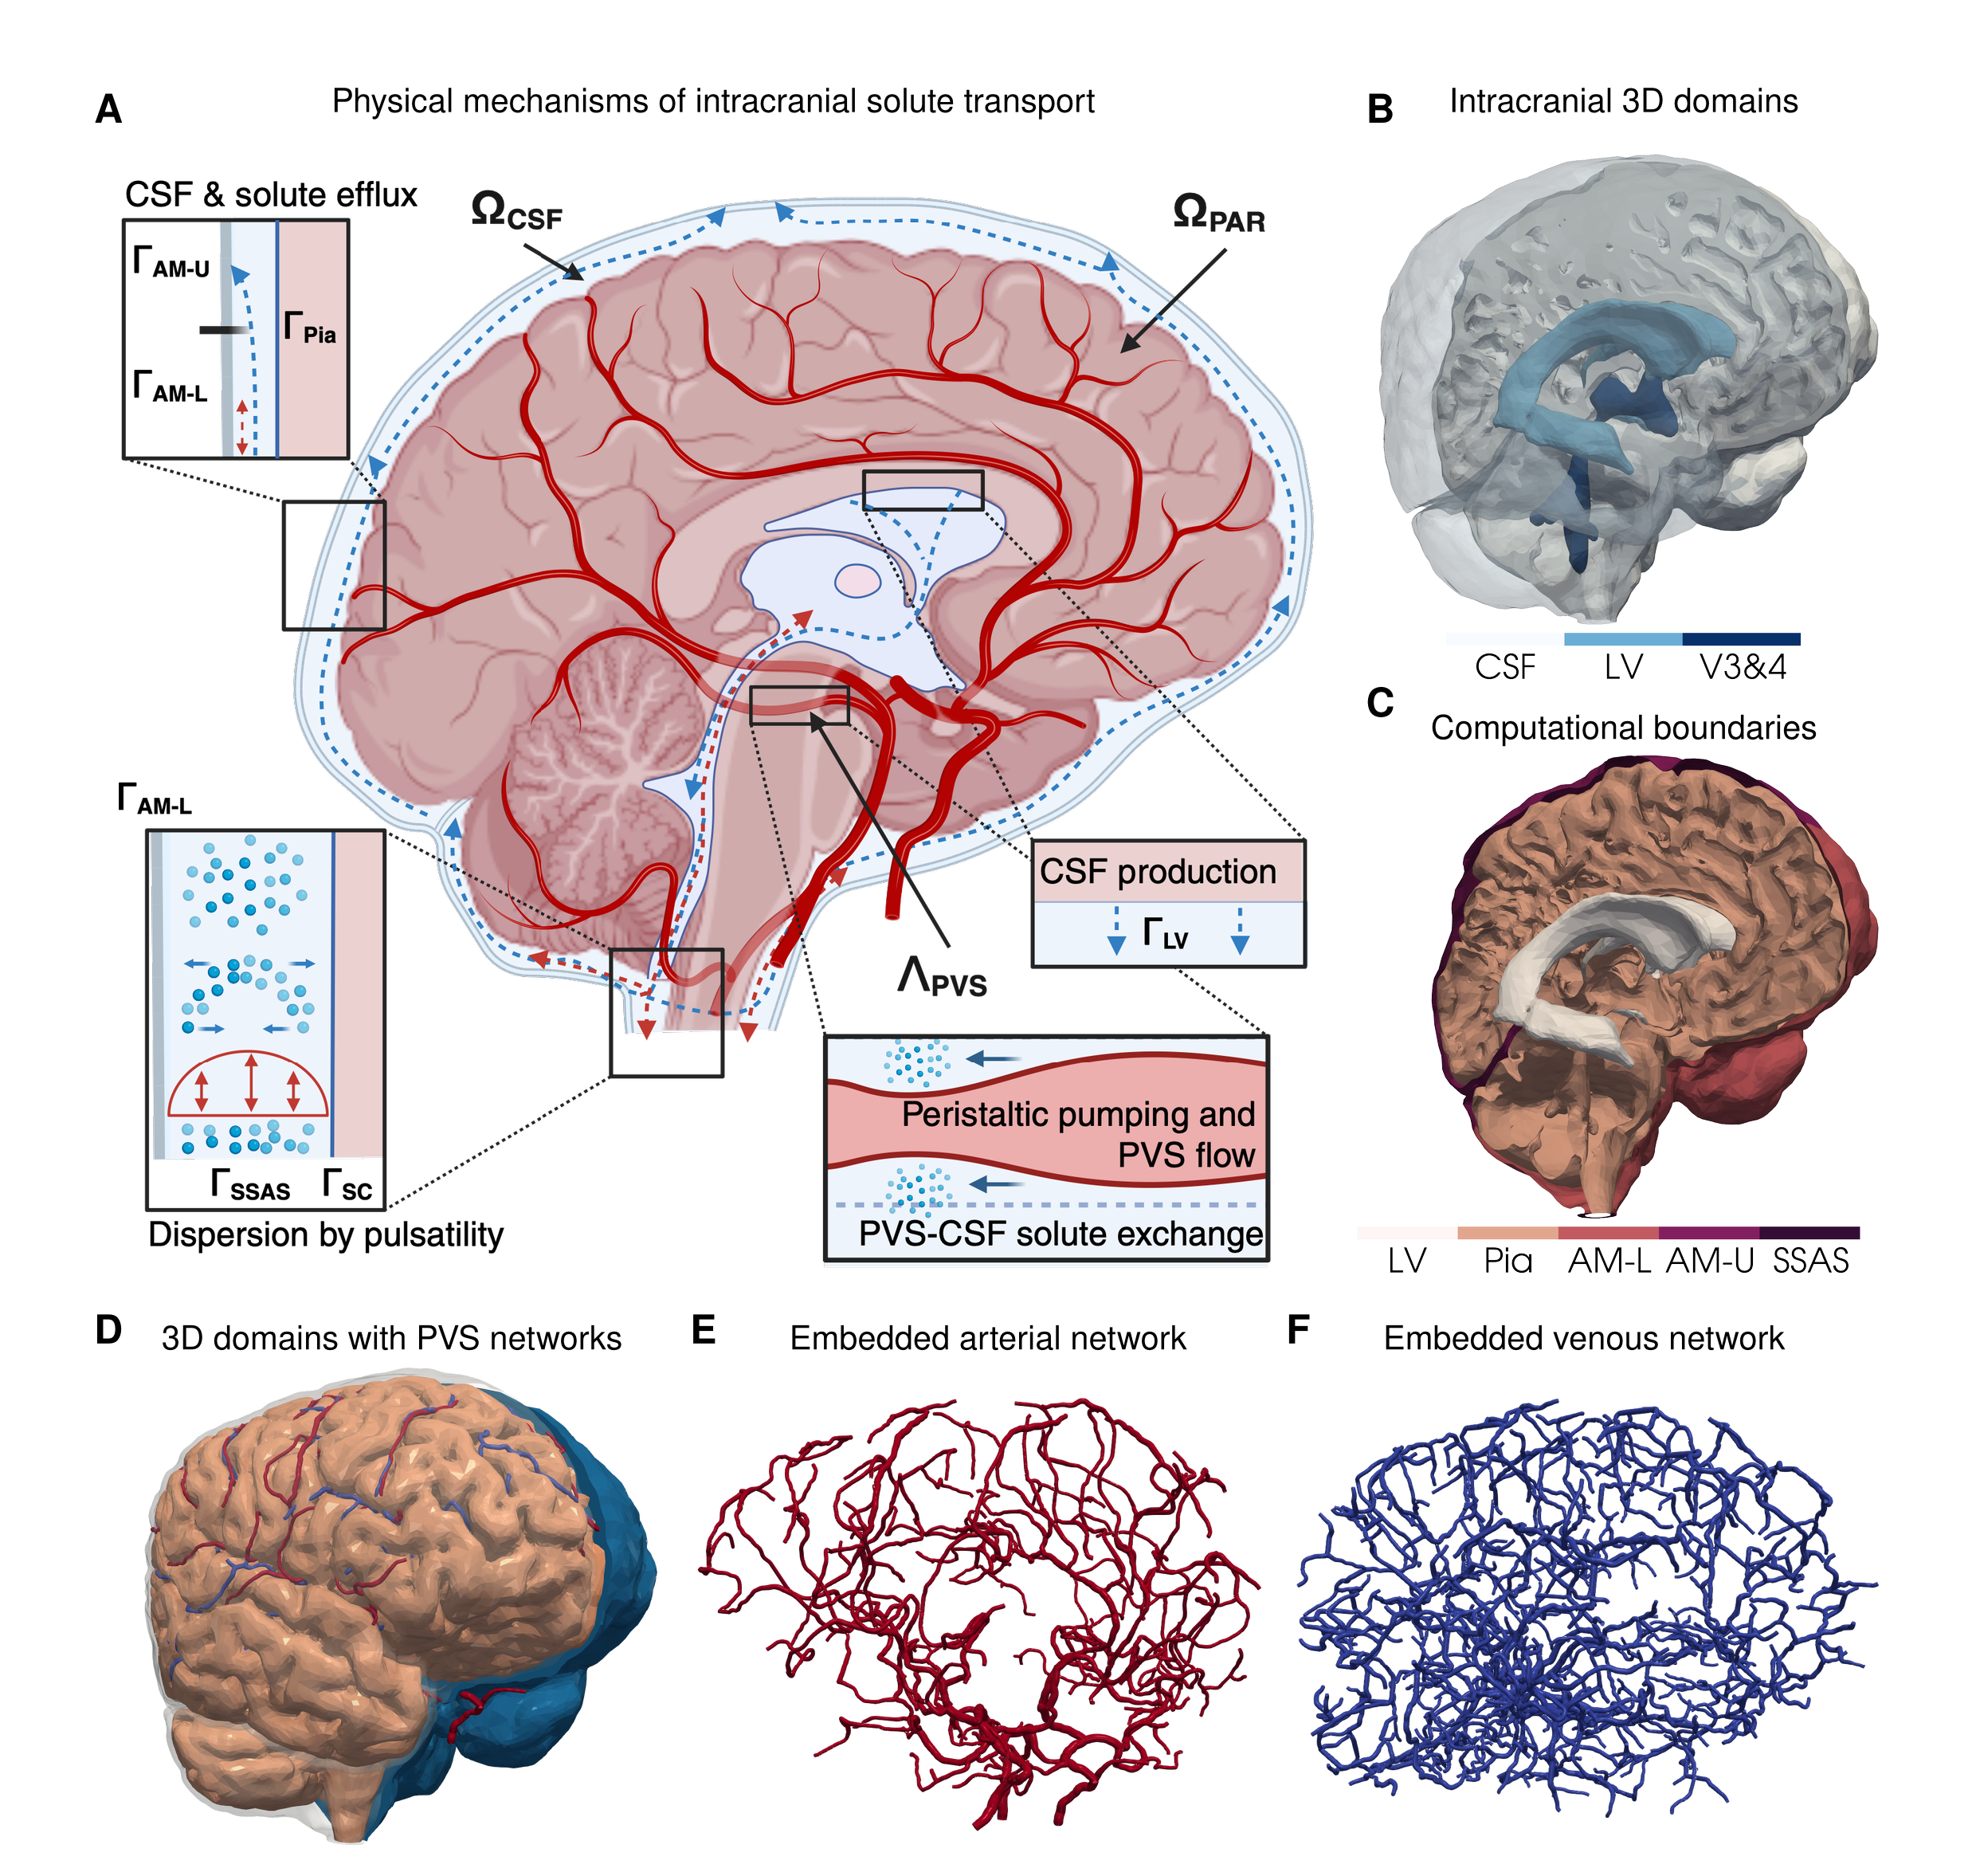
\includegraphics[width=0.7\textwidth]{figures/figure1.png}
     \DIFaddendFL \caption{ 
     \DIFaddbeginFL \textbf{\DIFaddFL{In-silico modelling of tracer transport in the PVS, SAS and parenchyma.}}
     \DIFaddendFL A)  \DIFaddbeginFL \DIFaddFL{Illustration of }\DIFaddendFL the  \DIFaddbeginFL \DIFaddFL{model geometry including the CSF-filled spaces }\DIFaddendFL ( ventricles  and SAS )  \DIFaddbeginFL \DIFaddFL{$\Omega_{\rm CSF}$, the parenchyma $\Omega_{\rm PAR}$ }\DIFaddendFL and \DIFaddbeginFL \DIFaddFL{the PVS surrounding arteries $\Lambda_{\rm artery}$ and veins $\Lambda_{\rm vein}$, as well as their }\DIFaddendFL interfaces \DIFaddbeginFL \DIFaddFL{and boundaries; 
     B) 3D rendering of the computational geometry}\DIFaddendFL : the  \DIFaddbeginFL \DIFaddFL{parenchyma}\DIFaddendFL ,  \DIFaddbeginFL \DIFaddFL{CSF }\DIFaddendFL ( \DIFaddbeginFL \DIFaddFL{clipped, blue}\DIFaddendFL ),  \DIFaddbeginFL \DIFaddFL{arterial network }\DIFaddendFL ( \DIFaddbeginFL \DIFaddFL{red}\DIFaddendFL )\DIFaddbeginFL \DIFaddFL{, }\DIFaddendFL and  \DIFaddbeginFL \DIFaddFL{venous network }\DIFaddendFL ( \DIFaddbeginFL \DIFaddFL{blue}\DIFaddendFL ); 
     C)  \DIFaddbeginFL \DIFaddFL{illustration }\DIFaddendFL of the  \DIFaddbeginFL \DIFaddFL{intrathecal tracer injection protocol}\DIFaddendFL ;  
     D)  \DIFaddbeginFL \DIFaddFL{in-silico predictions of tracer concentration after 1, 6, 12, and 24 hours }\DIFaddendFL ( \DIFaddbeginFL \DIFaddFL{opacity increasing linearly from 0 to 2 mmol/l}\DIFaddendFL ); 
     \DIFaddbeginFL \DIFaddFL{E) sagittal, coronal and axial view of in-silico tracer concentrations overlayed on T1-weighted MR image after 1, 6, 12 and 24\,h (low concentrations transparent, pial surface in pink, arachnoid membrane in cyan, and arteries in dark red); 
     F) average tracer concentration in each compartment over the first 24\,h; 
     G) total amount of tracer in each compartment over the first 24\,h.}\DIFaddendFL }
      \DIFaddbeginFL \label{fig:intrathecal}
\DIFaddendFL \end{figure}


 %DIF >  Reduced CSF pulsatility strongly shifts intracranial tracer distribution patterns
\DIFaddbegin \subsection*{\DIFadd{Can variations in CSF convection and dispersion shift these tracer distribution patterns?}} 

%DIF > % \begin{figure}%[h!]
%DIF > % \centering 
%DIF > % 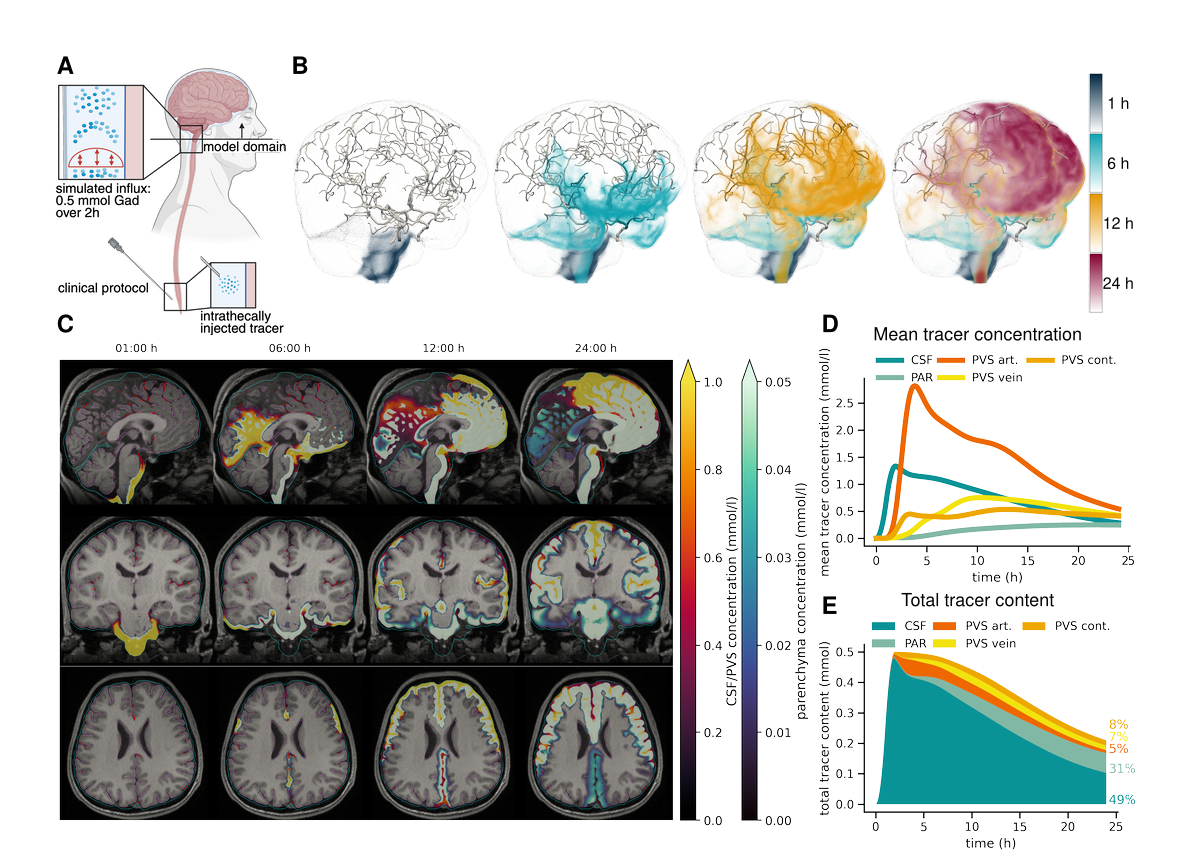
\includegraphics[width = 0.95\textwidth]{figures/figure2.png}
%DIF > % \caption{\textbf{The balance between CSF pulsatility and production shapes tracer distribution patterns.}
%DIF > % A) CSF spaces: the third and fourth ventricle (V3\&4), lateral ventricles (LV) and SAS; 
%DIF > % B) Boundaries and interfaces: the spinal subarachnoid space (SSAS), upper and lower arachnoid membrane (AM-U and AM-L), pia (Pia) and lateral ventricles (LV); 
%DIF > % C) Schematic of the CSF flow model; 
%DIF > % D) CSF flow induced by CSF production with outflow allowed across the
%DIF > % upper convexity (AM-U); 
%DIF > % }
%DIF > % \label{fig:csf}
%DIF > % \end{figure}
%DIF > % \begin{figure}
%DIF > % \ContinuedFloat
%DIF > % \caption{(\textbf{cont.})
%DIF > % E) Histograms of the production-induced CSF velocities in the SAS and third and fourth ventricle (V3 \& V4) in terms of the relative frequency of the mean flow speed in each computational cell weighted by its volume; 
%DIF > % F) CSF flow induced at peak systolic blood inflow; 
%DIF > % G) Cardiac-induced dispersion factor $R_c$;
%DIF > % H) CSF flow induced at peak respiratory expansion; 
%DIF > % I) Respiration-induced dispersion factor $R_r$, $D = (1 + R_c + R_r) D^{\rm Gad}$; J--M): Histograms of the cardiac-induced flow velocities (J),
%DIF > % cardiac-induced dispersion factors (K),
%DIF > % respiratory flow velocities (L), respiratory dispersion factor (M);
%DIF > % N--Q): sagittal, coronal and axial planes of tracer concentration after 12h for different model variations: baseline (N), no CSF production (O), low dispersion (P), and high dispersion (Q).
%DIF > % }
%DIF > % \end{figure}  

\DIFadd{Tracer distribution patterns observed }\DIFaddend after intrathecal injection
 differ substantially between subjects and  \DIFaddbegin \DIFadd{in conditions }\DIFaddend associated
with alterations in the pulsatile flow of CSF \DIFaddbegin \DIFadd{~\mbox{%DIFAUXCMD
\cite{ringstad2018brain,
  eide2021direction, eide2021impaired, eide2022altered}}\hskip0pt%DIFAUXCMD
. Cardiac and
respiratory pulsatility clearly also varies from subject to subject
and between }\DIFaddend physiological states.  \DIFaddbegin \DIFadd{Motivated by these observations, we
asked whether and how the tracer distribution patterns predicted by
our computational framework would be affected by changes in CSF
production or pulsatility.
%DIF > 
%DIF > % For the CSF dynamics in our baseline model, we combine the net
%DIF > % contribution to CSF flow induced by CSF production with the integrated
%DIF > % dispersive effects of cardiac and respiratory pulsatile CSF flow
%DIF > % (\Cref{fig:csf}A--C).
%DIF > 
%DIF > % Beginning with the advective, net flow field driven by CSF production,
%DIF > % we impose a constant CSF inflow of $400\,$ml/day across the surface of
%DIF > % the lateral ventricles. Simultaneously allowing for efflux across the
%DIF > % upper convexity yields a total CSF pressure drop of $26\,$mPa (0.00020
%DIF > % mmHg) (\Cref{fig:csf}D) with a maximum flow velocity of $1.85\,$mm/s
%DIF > % (in the aqueduct) and a mean velocity in the SAS of $2.6$\textmu m/s
%DIF > % (\Cref{fig:csf}E).
%DIF > 
To address this question, we introduce }\DIFaddend three variations of the
baseline  \DIFaddbegin \DIFadd{model: with }\DIFaddend (i) no CSF production, (ii) reduced
pulsatility \DIFaddbegin \DIFadd{/}\DIFaddend decreased dispersion, and (iii) higher
pulsatility \DIFaddbegin \DIFadd{/increased dispersion, respectively (\mbox{%DIFAUXCMD
\Cref{fig:csf}}\hskip0pt%DIFAUXCMD
)}\DIFaddend . We
computed the reduced and increased pulsatility scenarios by halving
and doubling the inflow rates associated with both cardiac and
respiratory pulsations \DIFaddbegin \DIFadd{(see Methods)}\DIFaddend , which changed the dispersion
factors by 0.25$\times$ and 4$\times$, respectively. Note that \DIFaddbegin \DIFadd{this
}\DIFaddend behaviour directly reflects the nature of our \DIFaddbegin \DIFadd{CSF model }\DIFaddend model: Stokes
flow is linear in its inflow boundary conditions, and the diffusion
enhancement factor is quadratic in the predicted pressure gradient.
 \DIFaddbegin 

\DIFadd{Without the convective contribution from }\DIFaddend CSF production, transport is
considerably delayed ( \DIFaddbegin \DIFadd{\fixme{\Cref{fig:csf}}}\DIFaddend ). Even after $12$ hours,
tracer remains in the subtentorial regions around the cerebellum, the
brain stem and in the surrounding CSF. Interestingly,  \DIFaddbegin \DIFadd{our model
instead predicts that the tracer will }\DIFaddend travel upwards through the
ventricular system, reaching the third ventricle after around $12$
hours. On the other hand,  \DIFaddbegin \DIFadd{in the model variation with reduced CSF
pulsatility}\DIFaddend , we observe rapid transport towards the upper convexity of
the cranium, as in the baseline model, but the tracer spreads
exclusively within the anterior regions ( \DIFaddbegin \DIFadd{\fixme{\Cref{fig:csf}}}\DIFaddend ). This
feature can be attributed to the CSF flow bifurcation posterior to the
ambient cistern ( \DIFaddbegin \DIFadd{\fixme{\Cref{fig:results1}}}\DIFaddend ): without sufficient
diffusion, the tracer is unable to cross into the posterior
SAS. Indeed, \DIFaddbegin \DIFadd{in the model variation }\DIFaddend with higher dispersion, the tracer
moves through the quadrigeminal cistern and further upwards into the
longitudinal fissure,  \DIFaddbegin \DIFadd{also spreading into }\DIFaddend the cerebellum
( \DIFaddbegin \DIFadd{\fixme{\Cref{fig:csf}}}\DIFaddend ).

\DIFaddbegin \begin{figure}%DIF > [h!]
\centering 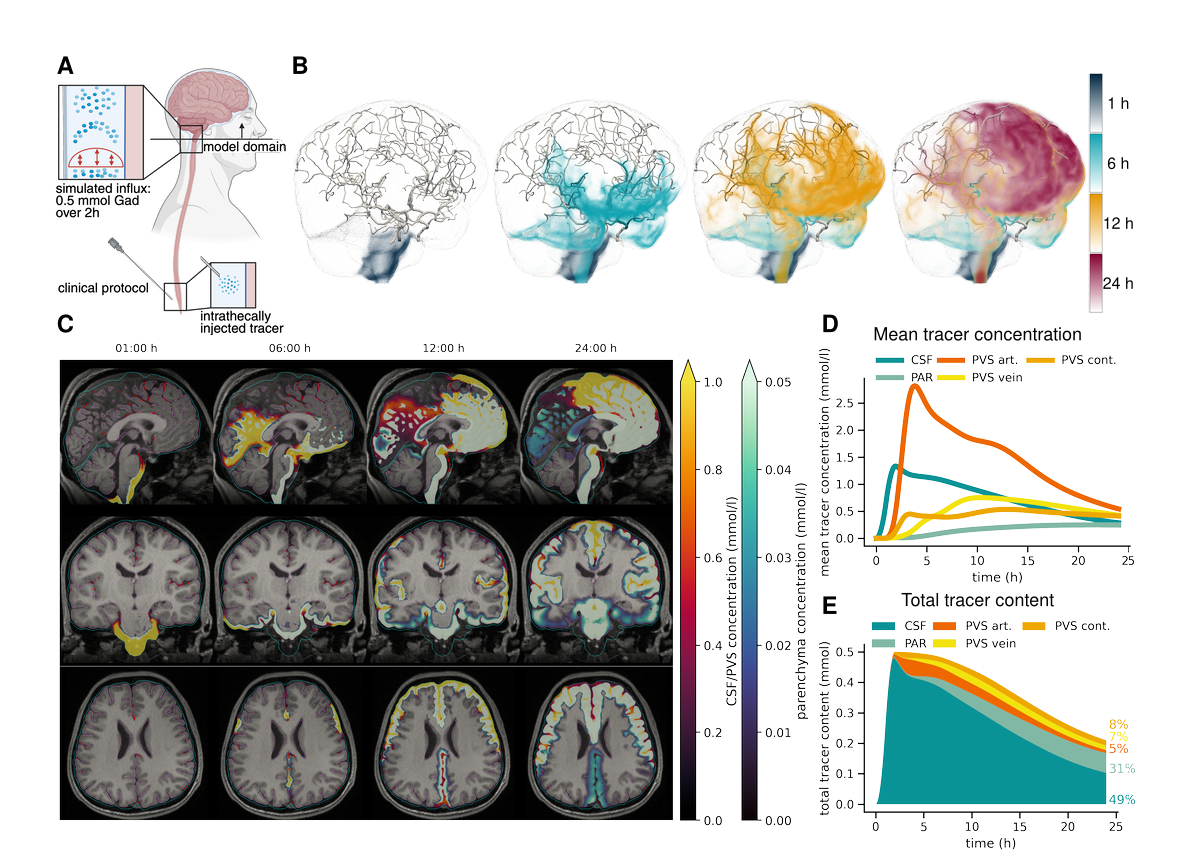
\includegraphics[width=0.8\textwidth]{figures/figure2.png}
\caption{\textbf{\DIFaddFL{Changes in the balance between convection and
    dispersion in the CSF spaces substantially alter computational
    predictions of tracer distribution patterns.}} \DIFaddFL{A) CSF flow induced
  by CSF production; B) Histograms of the production-induced CSF
  velocities in the SAS and third and fourth ventricle (V3 \& V4) in
  terms of the relative frequency of the mean flow speed in each
  computational cell weighted by its volume; C) Cardiac-induced
  dispersion factor $R_c$ with histogram in D); E) Respiration-induced
  dispersion factor $R_r$ with histogram in F). In the baseline model,
  A) represents the convective flow in the CSF spaces, while the
  factors $R_c$ in C) and $R_r$ in E) represent dispersion: $D = (1 +
  R_c + R_r) D^{\rm Gad}$.  G)--J): Sagittal, coronal and axial planes
  of tracer concentration after 12h for different model variations:
  baseline (G), no CSF production (H), low dispersion (I), and high
  dispersion (J).}}
\label{fig:csf}
\end{figure}

\DIFaddend \subsection*{ \DIFaddbegin \DIFadd{Can perivascular }\DIFaddend flow  \DIFaddbegin \DIFadd{shape }\DIFaddend and  \DIFaddbegin \DIFadd{accelerate }\DIFaddend molecular transport\DIFaddbegin \DIFadd{?}\DIFaddend }
\label{sec:pvs_flow_results}

%DIF >  FIXME: MER: This was the old one. Much better isn't it? 
%DIF > % The PVSs are recognized across species as critical pathways for solute
%DIF > % transport in and around the brain, and thus as potential targets for
%DIF > % enhancing brain drug delivery and metabolic waste clearance. However,
%DIF > % whether CSF flows more rapidly in PVSs and what the forces and
%DIF > % mechanisms required to drive such flow are, remain as key points of
%DIF > % debate~\cite{bohr2022glymphatic, van2024caa}. Motivated by
%DIF > % experimental observations in animal
%DIF > % models~\cite{iliff2012paravascular, iliff2013cerebral, mestre2018flow,
%DIF > %   bedussi2018paravascular}, there is now a remarkable body of
%DIF > % literature on modelling perivascular fluid flow and
%DIF > % transport~\cite{bilston2003arterial, asgari2016glymphatic,
%DIF > %   rey2018pulsatile, daversin2020mechanisms, sharp2019dispersion,
%DIF > %   thomas2019fluid, kedarasetti2020functional, kedarasetti2020arterial,
%DIF > %   troyetsky2021dispersion, martinac2021phase, gjerde2023directional,
%DIF > %   nozaleda2024arterial}. Here, we ask how these proposed mechanisms
%DIF > % would translate from idealized geometries to human vascular networks
%DIF > % and moreover, evaluate their integrated effect in the context of
%DIF > % intracranial solute transport.
\DIFaddbegin 

\DIFaddend The PVSs are recognized across species as critical pathways for solute
transport in and around the brain, and thus as potential targets for
enhancing brain  \DIFaddbegin \DIFadd{solute transport }\DIFaddend and metabolic waste clearance. However,
whether CSF flows more rapidly in  \DIFaddbegin \DIFadd{human PVSs stands as an open
question~\mbox{%DIFAUXCMD
\cite{bohr2022glymphatic, van2024caa,
  kipnis2025resolving}}\hskip0pt%DIFAUXCMD
. In light of this, we asked to what extent our
predicted tracer distributions would be affected by the }\DIFaddend flow in \DIFaddbegin \DIFadd{the
PVSs. Specifically, we here introduce a model variation with
substantially higher net flow in }\DIFaddend the PVS \DIFaddbegin \DIFadd{, by adding the contribution
from strong ultraslow vasomotion to that from }\DIFaddend the cardiac pulse wave
 \DIFaddbegin \DIFadd{(\fixme{\Cref{fig:pvs}X, Y}), and compare with the baseline model.
}\DIFaddend 

 In both models, tracers were first observed at the basal artery after
48 minutes ( \DIFaddbegin \DIFadd{\mbox{%DIFAUXCMD
\Cref{fig:high_low_pvs}}\hskip0pt%DIFAUXCMD
}\DIFaddend A), defined by their first-time
arrival (FTA), the time at which the concentration first exceeds $0.1$
mmol/l. At all upstream locations along the middle cerebral arteries
(MCAs) and anterior cerebral artery (ACA), we found substantially
reduced FTAs with higher  \DIFaddbegin \DIFadd{perivascular flow (\mbox{%DIFAUXCMD
\Cref{fig:high_low_pvs}}\hskip0pt%DIFAUXCMD
}\DIFaddend B), up to
2.5 hours earlier in the left M2 segment of the MCA. PVS
concentrations peaked before the surrounding tissue (0:48h vs 1:12h at
the MCA and 1:00h vs 1:48h at MCA2) with high PVS flow, while these
peaks occurred nearly simultaneously in the baseline model. The
earlier appearance and the delay in time-to-peak between the PVS and
surrounding tissue clearly indicates the directionality of tracer
 \DIFaddbegin \DIFadd{movement in our model }\DIFaddend -- it first arrives in the PVS and subsequently
spreads into the tissue and SAS ( \DIFaddbegin \DIFadd{\mbox{%DIFAUXCMD
\Cref{fig:high_low_pvs}}\hskip0pt%DIFAUXCMD
}\DIFaddend C, D), and
especially so with higher  \DIFaddbegin \DIFadd{perivascular }\DIFaddend flow. These observations also hold on an
aggregated level: computing the total amount of tracer in the PVS as a
function of the distance to the arterial network roots, we find
accelerated tracer transport with higher  \DIFaddbegin \DIFadd{perivascular }\DIFaddend flow, especially at
earlier time points (2--9 hours) ( \DIFaddbegin \DIFadd{\mbox{%DIFAUXCMD
\Cref{fig:high_low_pvs}}\hskip0pt%DIFAUXCMD
}\DIFaddend E). Moreover,
differences in tracer transport along the PVS translate to altered
 \DIFaddbegin \DIFadd{distribution }\DIFaddend patterns on the whole-organ scale. For instance, after
4-6 hours, the faster-moving tracer in the PVS is clearly visible in
the space adjacent to the PVS of the ACA, MCA, and other arteries
( \DIFaddbegin \DIFadd{\mbox{%DIFAUXCMD
\Cref{fig:high_low_pvs}}\hskip0pt%DIFAUXCMD
}\DIFaddend G). In contrast, there are no clear signs of
early  \DIFaddbegin \DIFadd{appearance of tracer }\DIFaddend surrounding the PVS in the baseline model
( \DIFaddbegin \DIFadd{\mbox{%DIFAUXCMD
\Cref{fig:high_low_pvs}}\hskip0pt%DIFAUXCMD
}\DIFaddend F).

A  \DIFaddbegin \DIFadd{related }\DIFaddend question is whether early  \DIFaddbegin \DIFadd{appearance of tracer in the PVS
}\DIFaddend could be the result of increased dispersion rather than net flow in
the PVS
\cite{asgari2016glymphatic,sharp2019dispersion,bojarskaite2023sleep,asgari2016glymphatic,troyetsky2021dispersion}. Interestingly,
\DIFaddbegin \DIFadd{in our model, }\DIFaddend even increasing the dispersion factor by $100 \times$ in
the PVS, induced only minor changes in the global spreading rate
compared to the baseline ( \DIFaddbegin \DIFadd{\mbox{%DIFAUXCMD
\Cref{fig:high_low_pvs}}\hskip0pt%DIFAUXCMD
}\DIFaddend F, H) .

 %DIF > Imposing the pressure field induced by CSF production at the
%DIF > periarterial network ends induces slow steady CSF flow of variable
%DIF > direction in these PVSs, with an average velocity of 0.08 \textmu m/s
%DIF > (antegrade) and a maximum velocity of 0.55 \textmu m/s (\Cref{fig:pvs}B).

%DIF > % Applying a semi-analytic model
%DIF > % of the net flow induced by peristalsis in perivascular
%DIF > % networks~\cite{gjerde2023directional} (see Methods), we estimate that
%DIF > % the cardiac pulse wave alone, traveling at a frequency of 1 Hz with a
%DIF > % wavelength of 2.0 m and a 1\% wall displacement~\cite{jung2021novel},
%DIF > % will induce mainly antegrade PVS flow with an average net velocity of
%DIF > % 0.92 \textmu m/s while reaching up to 7.31 \textmu m/s near larger,
%DIF > % ventral vessels such as the MCA (\Cref{fig:pvs}D,E). The same theory
%DIF > % predicts that strong ultraslow vasomotions, if traveling antegrade at
%DIF > % 0.1Hz with a wavelength of 0.02 m and a 10\%
%DIF > % displacement~\cite{broggini2024long}, will induce both retrograde and
%DIF > % antegrade net PVS flow with an average velocity of 13.05 \textmu m/s
%DIF > % and maximum velocity 54.44 \textmu m/s (\Cref{fig:pvs}D,F).
\DIFaddbegin 

\DIFaddend \begin{figure}
    \centering
    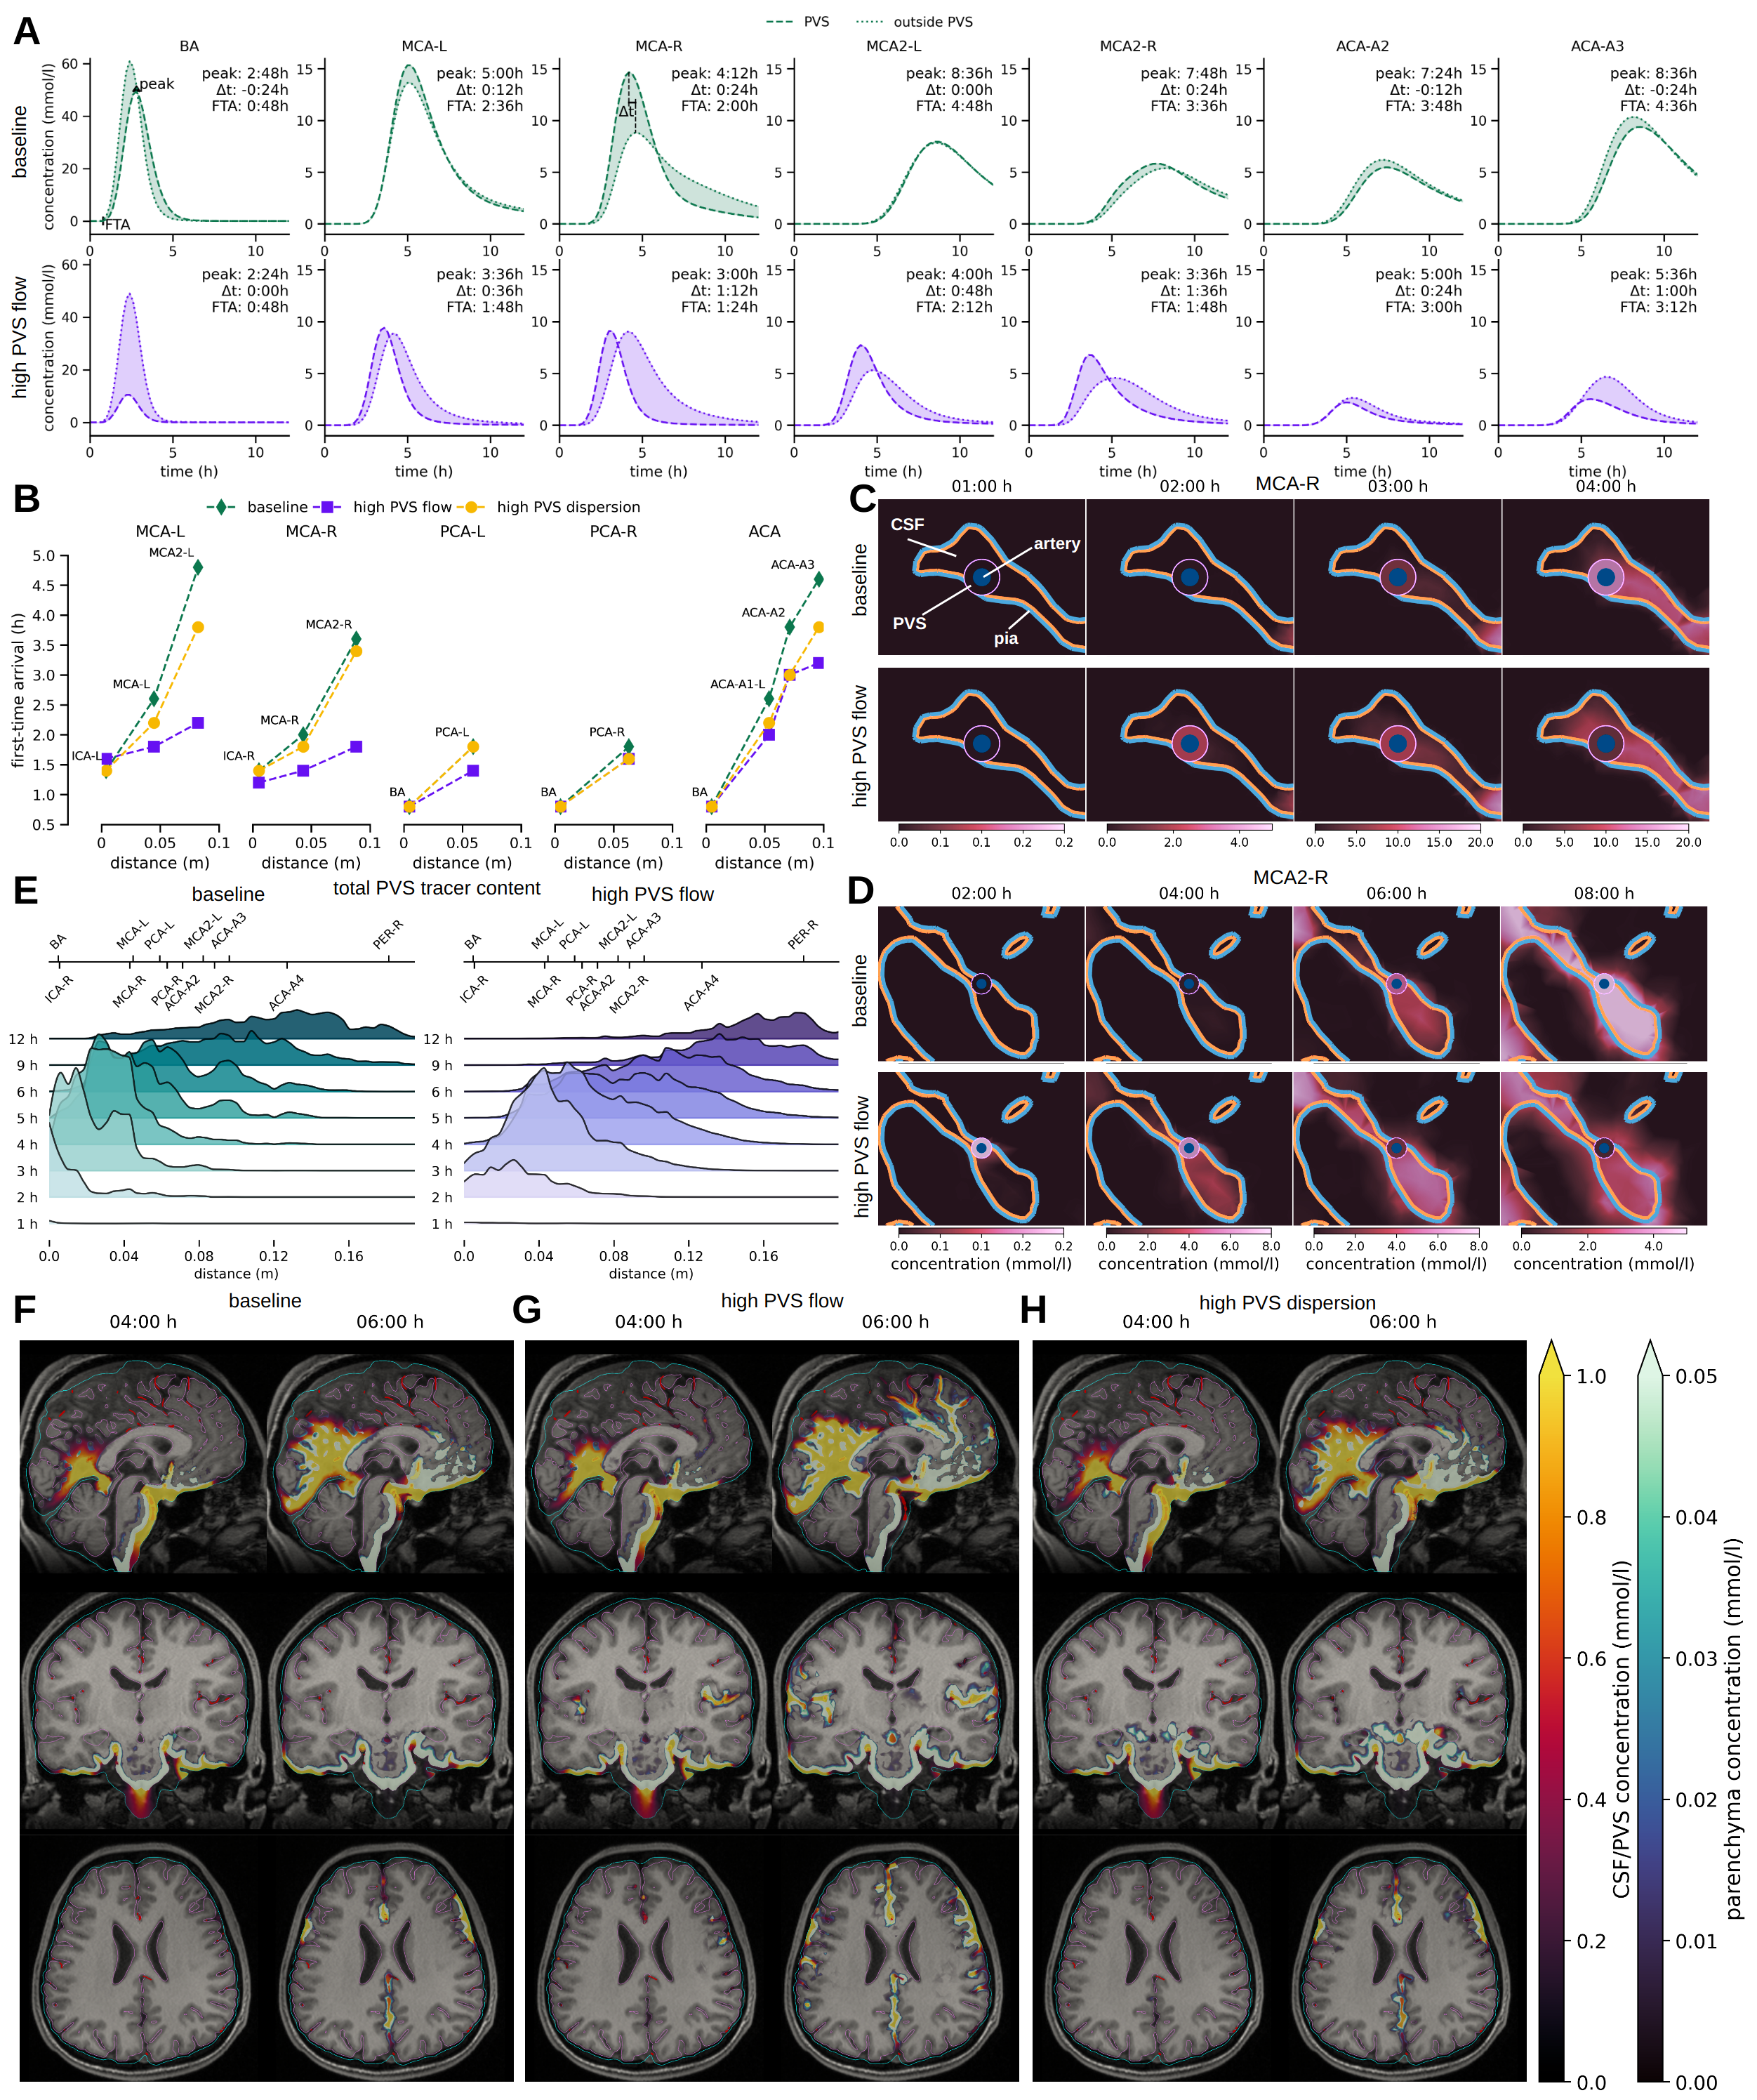
\includegraphics[width=0.99\textwidth]{figures/figure3b.png}
    \caption{\textbf{Perivascular flow shapes and accelerates molecular transport.}
    A) Comparison of mean tracer concentration in the PVS and over the outer PVS surface at key locations of the arterial tree, for the baseline (lower) and high PVS flow (upper) models, with labels: ``peak'': time-to-peak (h), ``$\Delta t$'': time difference between peaks (h), and ``FTA'': first-time tracer arrival (h).
    B) first-time arrival for the main trunks of the periarterial network over the distance from the closest network root node (BA, ICA-R or ICA-L for the baseline, the high PVS flow and the high PVS dispersion models);}
     \DIFaddbeginFL \label{fig:high_low_pvs}
\DIFaddendFL \end{figure}
\begin{figure}
\ContinuedFloat
\caption{(\textbf{cont.})
    C, D) 2D slices showing zoom-in on the region surrounding the MCA-R and MCA2-R for the baseline (upper) and high PVS flow (lower) models. Innermost circle indicates the artery (blue), the surrounding annulus is the PVS (color represents concentration value), the surroundings are parenchyma and/or CSF spaces, separated by the pia (blue: towards the parenchyma, pink: towards the CSF));  
    E) Total amount of tracer in the periarterial spaces as a function of the distance to the nearest network root over time for the baseline (left) and the high PVS flow (right) models;
    F--H) sagittal (upper) and coronal (lower) views of the simulated tracer concentrations overlayed on the T1-weighted MR image after 4 and 6h for the baseline (K), high PVS flow (L) and high PVS dispersion (M) models (concentration opacity linearly increasing with concentration value, pial surface outlined in pink, arachnoid membrane in cyan, and arteries in dark red). An interactive visualization of the baseline and the high PVS flow model can be found \href{https://baseline-pvs-flow.surge.sh/}{here}, and \href{https://high-pvs-flow.surge.sh/}{here}.}
\end{figure}  

\subsection*{Structural versus functional compartmentalization of perivascular spaces}

Human and rodent observations indicate that tracers concentrate in perivascular spaces surrounding the pial and subarachnoid vasculature \cite{zhang1990interrelationships,zhang1992directional, bedussi2017paravascular, mestre2018flow, bedussi2018paravascular, eide2024functional}. However, it remains unclear whether such  \DIFaddbegin \DIFadd{distribution }\DIFaddend patterns necessitate a structural barrier, such as a membrane with limited permeability, or if the patterns could result from enhanced flow or mixing in these areas alone. We therefore next investigate how the permeability of the interface between the PVS and the surrounding CSF affects tracer  \DIFaddbegin \DIFadd{distribution }\DIFaddend around the major arterial trunks \DIFaddbegin \DIFadd{in our model }\DIFaddend (\Cref{fig:compartmentalization}A--B). To this end, we compare models with high and low permeabilities, representing a highly permeable PVS-CSF interface (functional compartmentalization) and a less permeable interface (structural compartmentalization), respectively. For the low permeability model, we set the permeability to $3.8 \cdot 10^{-7}\,$m/s, consistent with previous estimates for the endfoot sheath surrounding penetrating arterioles \cite{koch2023estimates}, which we consider to be a lower bound for the surface PVS-CSF permeability. For the high permeability model, we increase this permeability by a factor of 100. We emphasize that, for both scenarios, we  \DIFaddbegin \DIFadd{apply }\DIFaddend the high PVS flow  \DIFaddbegin \DIFadd{model as described }\DIFaddend in the previous section. 

At the basal artery (BA), tracer appears within one hour in the surrounding CSF in both models (\Cref{fig:compartmentalization}C, E). With a more permeable PVS-CSF interface, tracer quickly crosses from the CSF into the PVS, resulting in similar peak concentrations of 25\,mmol/l in the PVS and at its outer surface, while values up to 50\,mmol/l are attained in the vicinity. In contrast, the low permeability model exhibits substantially lower perivascular tracer  \DIFaddbegin \DIFadd{concentrations}\DIFaddend , with a maximum concentration of 10\,mmol/l after approximately two hours.
%The high permeability model allows for more tracer crossing into the PVS, leading to higher concentrations further downstream. Notably, crossover into the parenchyma is also observed, most clearly at 4 hours.
For the middle cerebral arteries (MCA-R and MCA-L), tracer appears
first in the PVS in both models (\Cref{fig:compartmentalization}D, E),
though with higher concentrations in the high permeability model (up
to 24 mmol/l). We also observe that the higher permeability allows the
tracer to leak out of the PVS and spread within the Sylvian fissure to
a greater extent. With a small delay, more tracer appears via
  the CSF pathway (\Cref{fig:compartmentalization}D). At the anterior cerebral artery (ACA-A2), the first tracer arrival in the PVS occurs after 3 hours, with a peak at 5 hours. The concentration peak in the PVS is tailed by a higher peak in the CSF (\Cref{fig:compartmentalization}E), indicating tracer arrival through a second pathway; i.e., directly through the CSF-filled space outside of the PVS. Similar patterns are observed for ACA-A3.

Summarizing and quantifying these \DIFaddbegin \DIFadd{model }\DIFaddend observations
(\Cref{fig:compartmentalization}F), we find that neither the time of
first arrival nor the time-to-peak are substantially affected by the
PVS-CSF permeability at any of the periarterial segments considered
(BA, MCAs, ACAs). However, the concentration difference between the
PVS and its surrounding CSF quickly decreases with higher
permeability, as does the time lag between the concentration peaks in
these domains. Thus, \DIFaddbegin \DIFadd{in our model, }\DIFaddend fast transport along the PVS is not
contingent upon a structural compartmentalization of the PVS, whereas
a sharp concentration gradient between PVS and CSF is unlikely without
a restricting barrier.
\begin{figure}
    \centering
    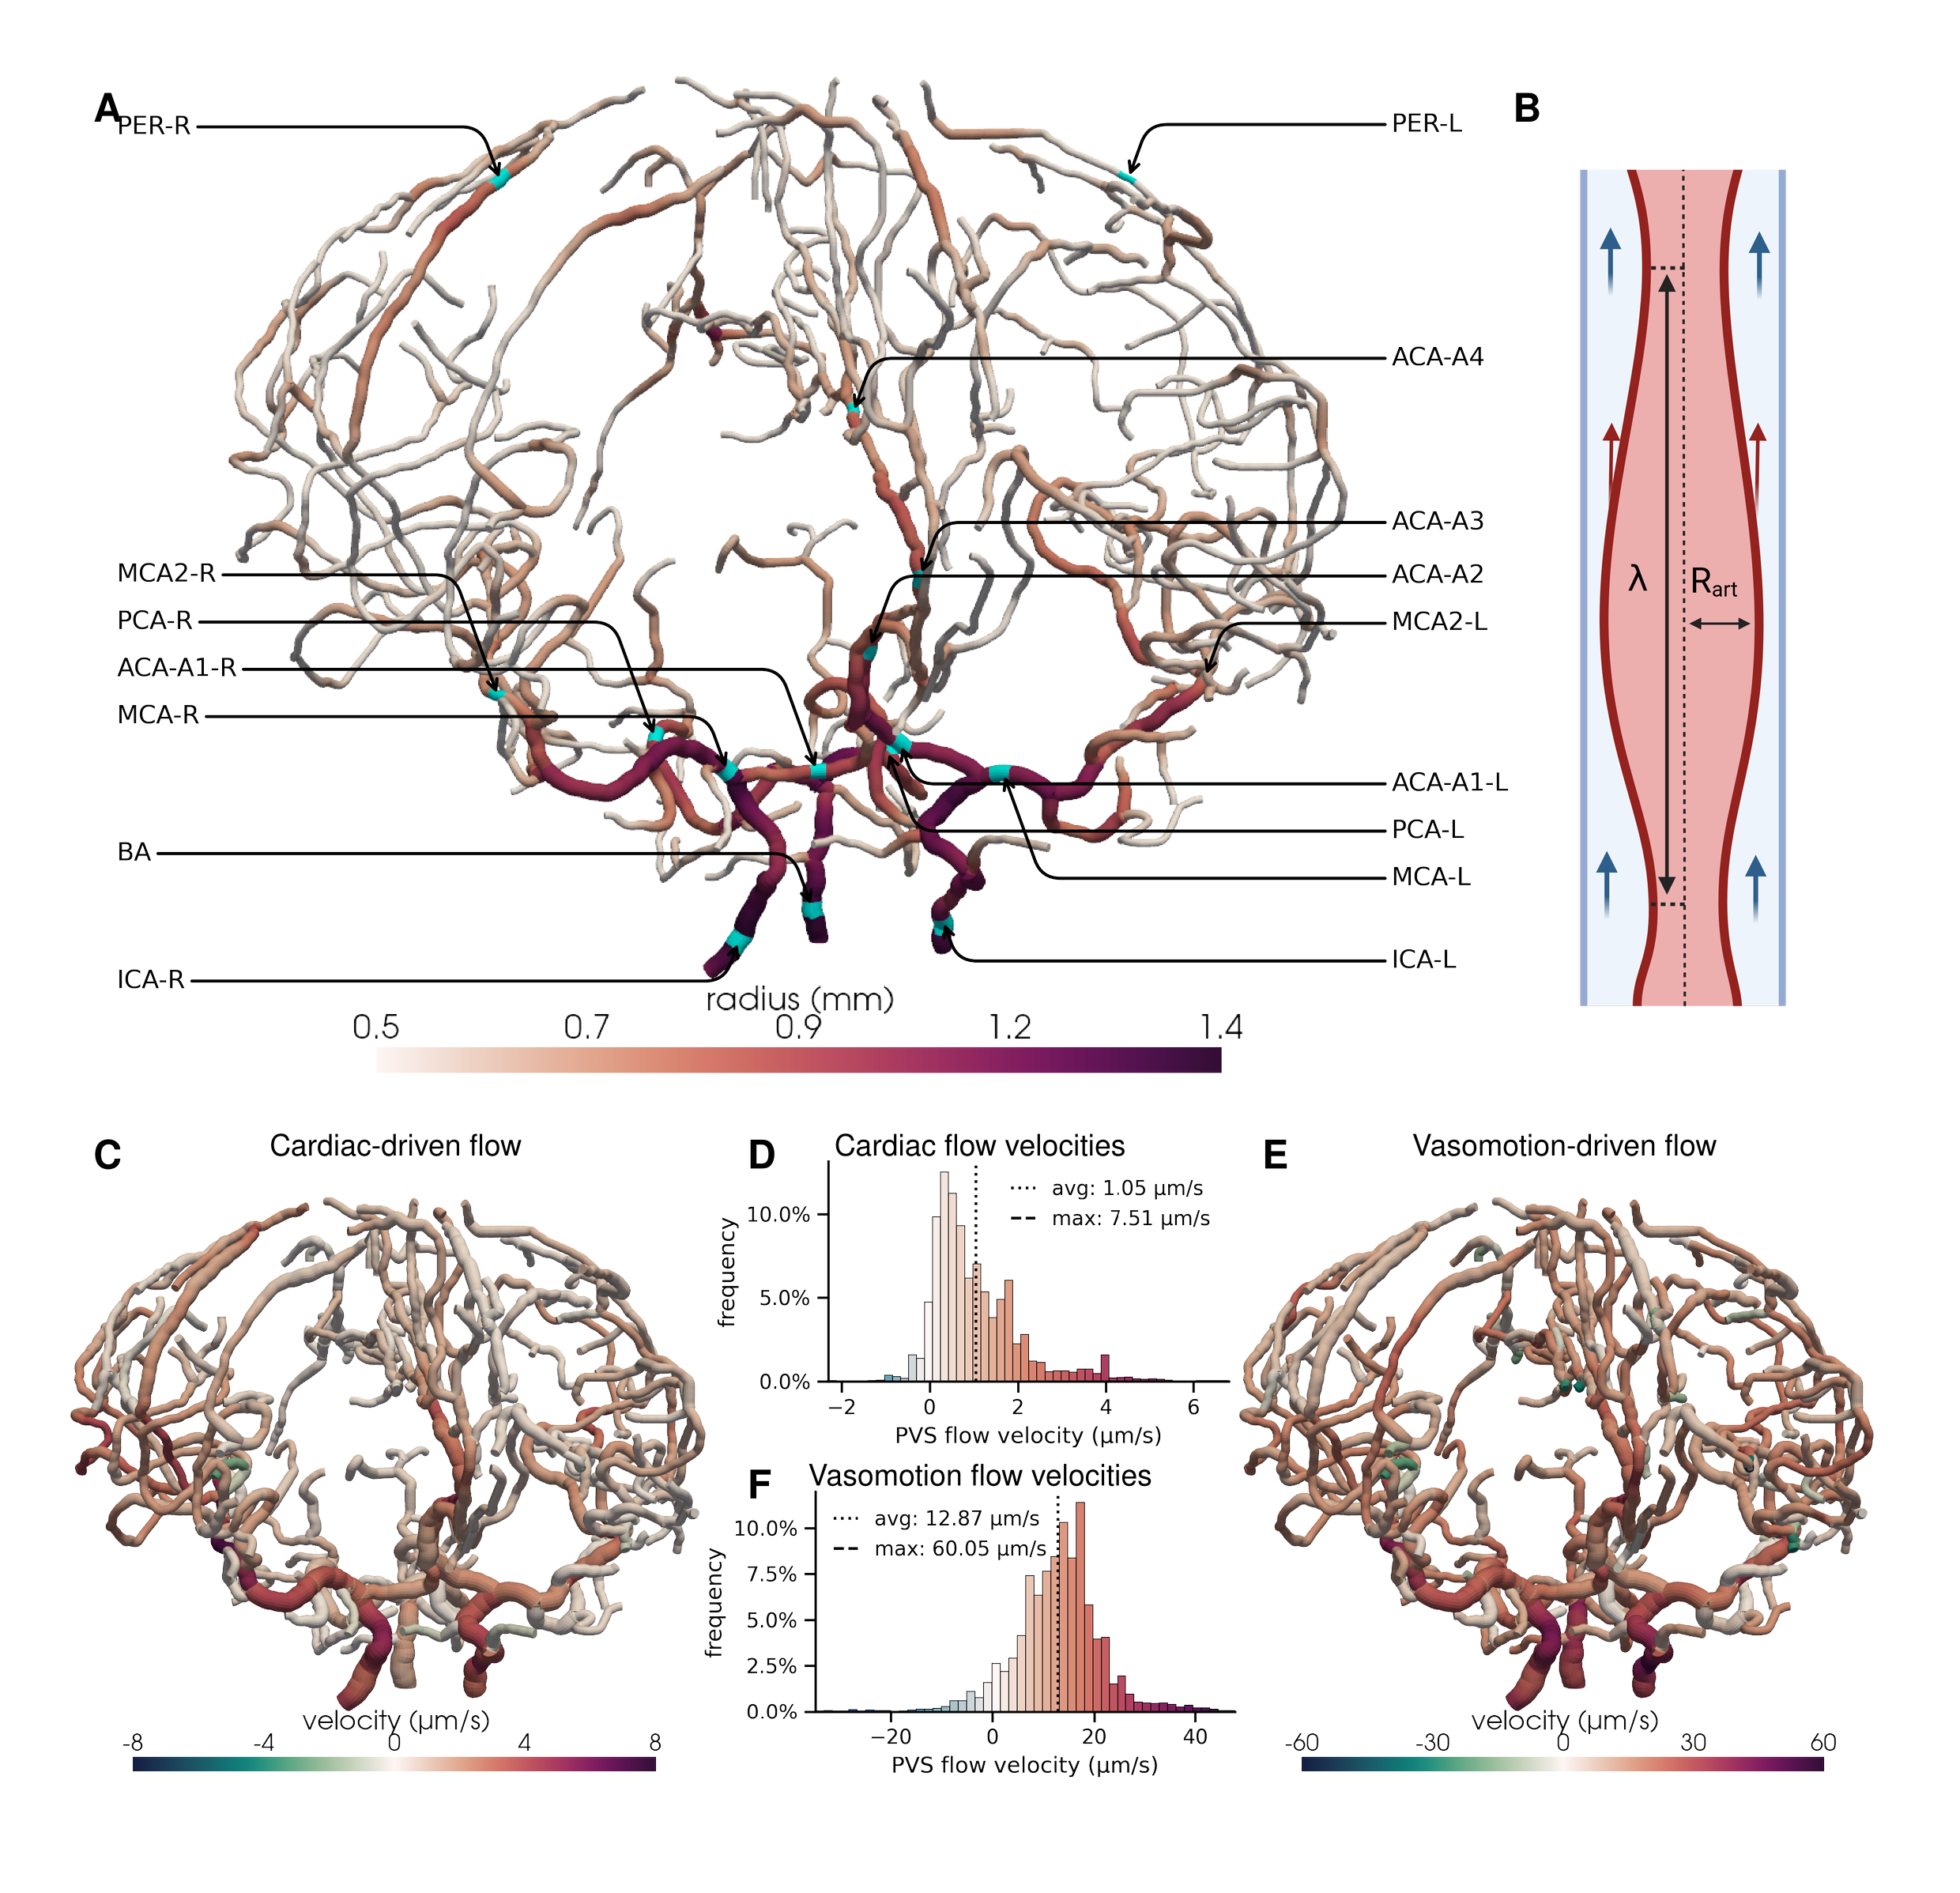
\includegraphics[width=0.95\textwidth]{figures/figure4.png}
    \caption{ \DIFaddbeginFL \textbf{\DIFaddFL{Does early appearance of tracer in the PVS rely on a structural compartmentalization of the PVS?}}
    \DIFaddendFL A)  \DIFaddbeginFL \DIFaddFL{In our model, the }\DIFaddendFL PVS-CSF membrane permeability regulates the exchange of solutes between the PVS and surrounding CSF spaces; 
    B) The arterial network with highlighted regions of interest; 
    C) 2D slices showing zoom-in to the region surrounding the basal artery after 1, 2, 3, and 4 hours for a low (above) and high (below) PVS-CSF permeability model. Innermost circle indicates the artery (blue), the surrounding annulus is the PVS (color represents concentration value), the surroundings are parenchyma and/or CSF spaces, separated by the pia (blue: towards the parenchyma, pink: towards the CSF). The cutting planes are normal to the blood vessels;
    D) As in (C) for regions surrounding (from upper to lower) the ACA-A3, ACA-A2, MCA-R and MCA-L segments;}
    \label{fig:compartmentalization}
\end{figure}
\begin{figure}
\ContinuedFloat
\caption{(\textbf{cont.})
E) Comparison of mean tracer concentration in the PVS (dashed) and over the
outer PVS surface (dotted) for the BA, MCA-R, MCA-L, ACA-2, and ACA3 segments over time for the high (purple) and low permeability (yellow) models;
F) Effect of varying the PVS-CSF permeability on first-time-of-arrival (FTA), time difference ($\Delta t$) between concentration peaks in the PVS and surrounding tissue, time of PVS peak concentration, PVS peak concentration and difference in peak concentration between PVS and surrounding tissue.}
\end{figure}

\subsection*{ \DIFaddbegin \DIFadd{Will dilated }\DIFaddend PVSs in the SAS  \DIFaddbegin \DIFadd{impact the }\DIFaddend intracranial tracer  \DIFaddbegin \DIFadd{distribution?}\DIFaddend }

Idiopathic normal pressure hydrocephalus (iNPH), a dementia subtype,
is associated with enlarged PVS in the SAS and impaired periarterial
and parenchymal tracer transport~\cite{eide2024functional}. More
generally, enlarged PVSs are associated with a range of
pathophysiogical conditions and cognitive
decline~\cite{bown2022physiology}. A  \DIFaddbegin \DIFadd{natural }\DIFaddend question is thus whether
enlarged PVSs alone leads to delayed perivascular and intracranial
tracer  \DIFaddbegin \DIFadd{spread.
}

\DIFaddend To address this question from a fluid and transport dynamics
perspective, we  \DIFaddbegin \DIFadd{consider a final model variation in which we examine
the predicted }\DIFaddend effect of perivascular dilation on  \DIFaddbegin \DIFadd{perivascular }\DIFaddend flow velocities
and tracer  \DIFaddbegin \DIFadd{distribution }\DIFaddend patterns (\Cref{fig:enlargement}A).  \DIFaddbegin \DIFadd{We again
compute cardiac }\DIFaddend and vasomotion-induced net  \DIFaddbegin \DIFadd{perivascular }\DIFaddend flow velocities, but
now in a  \DIFaddbegin \DIFadd{periarterial }\DIFaddend geometry with an increased outer radius ($R^{\rm
  dilated}_2 = 3 R_1$) compared to the previous ($R^{\rm control}_2 =
2 R_1$), which corresponds to a $2.67 \times$ increase in PVS
cross-section area.
%% \begin{align*}
%%   A_1 = \pi (R_2^2 - R_1^2) = \pi (2^2 R_1^2 - R_1^2) = 3 \pi R_1^2 \\
%%   A_2 = \pi (\hat{R}_2^2 - R_1^2) = \pi (3^2 R_1^2 - R_1^2) = 8 \pi R_1^2 \\
%%   A_2 / A_1 = 8/3 = 2.76
%% \end{align*}
 \DIFaddbegin \DIFadd{With dilated PVSs, the }\DIFaddend peristaltic pumping becomes considerably
less effective: the cardiac and vasomotion-induced net CSF flow
velocities drop from a mean of 0.92 \textmu m/s to 0.17 \textmu m/s
and from 13.05 \textmu m/s to 2.33 \textmu m/s, respectively
(\Cref{fig:enlargement}B--D). In  \DIFaddbegin \DIFadd{turn, this }\DIFaddend alters the tracer  \DIFaddbegin \DIFadd{spread }\DIFaddend within the dilated
PVS. Notably, we observe later tracer arrival in all MCA segments,
with up to 96 min later arrival in the MCA2s for the high PVS flow
scenario (\Cref{fig:enlargement}E, F). For the  \DIFaddbegin \DIFadd{model without }\DIFaddend vasomotion-induced  flow, the effect is less
pronounced in the MCA but clearly persists and is evident in the MCA2s
(\Cref{fig:enlargement}F). Finally, we note that the larger volume of
the dilated PVS results in a greater total accumulation of tracer in
the PVS from 3--24 hours and reduced  \DIFaddbegin \DIFadd{amounts of tracer in }\DIFaddend the
parenchyma at 6 and 12 h, while the mean PVS concentration is
initially lower, but later exceeds the baseline model
(\Cref{fig:enlargement}G,H).
\begin{figure}
    \centering
    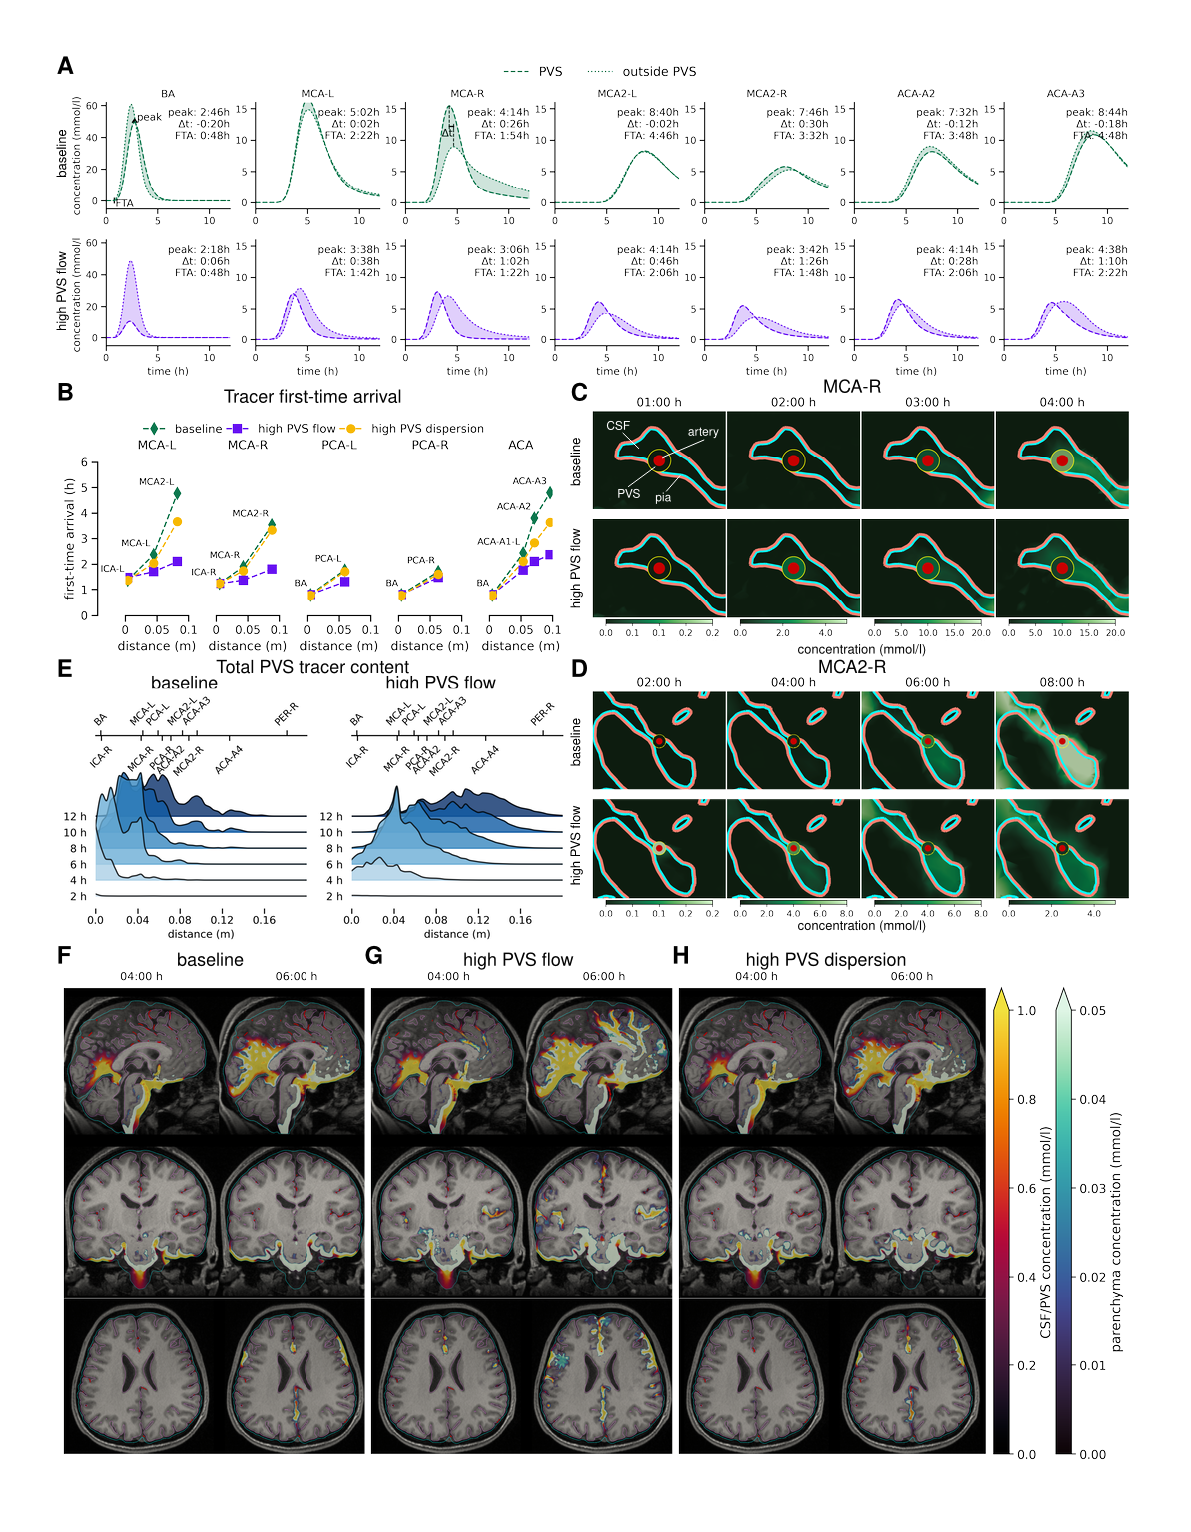
\includegraphics[width=1 \textwidth]{figures/figure5.png}
\caption{\textbf{PVS enlargement in the SAS reduces net PVS flow and delays tracer transport}
A) Modelling dilated PVS in the SAS by extending the outer PVS boundaries;
B) mean and max PVS flow velocities with normal/control and dilated PVS;
C--D) 3D rendering of vasomotion-induced PVS flow in the normal (C) and dilated (D) periarterial networks; 
E) 2D slices showing zoom-in to the region surrounding the MCA-R after 1, 2, 3, and 4\,h with normal (lower) and dilated (upper) PVS. Innermost circle indicates the artery (blue), the surrounding annulus is the PVS (color represents concentration value), the surroundings are parenchyma and/or CSF spaces, separated by the pia (blue: towards the parenchyma, pink: towards the CSF).The cutting plane is normal to the blood vessel; 
F) First-time arrival for different branches of the arterial tree for the baseline model (with pressure-driven and cardiac-induced net PVS flow) and the high PVS flow model (also including vasomotion-induced net PVS flow) for normal and dilated PVS;
G) total tracer content in the CSF, parenchyma and arterial and venous PVS at 1,3,6,12 and 24\,h for the four models from F;
H) mean concentration in the CSF, parenchyma and arterial and venous PVS over time for the four models from F.
}
    \label{fig:enlargement}
\end{figure}

\section*{Discussion}

%% Summary of findings
We have presented  \DIFaddbegin \DIFadd{an }\DIFaddend in-silico  \DIFaddbegin \DIFadd{modelling framework for solute
transport }\DIFaddend in human intracranial spaces,  \DIFaddbegin \DIFadd{informed by multi-modal
structural MRI, and integrating transport mechanisms across spatial
and temporal scales. To demonstrate its features and relevance, we
have presented a series of simulation scenarios relating to
intracranial distribution of an gadolinium-based contrast agent after
intrathecal injection, exploring }\DIFaddend the influence of CSF space and
(peri)vascular morphology, physiological factors such as cardiac and
respiratory pulsatility, as well as of pathological conditions such as
enlarged PVSs in the SAS.  \DIFaddbegin \DIFadd{In our simulations, }\DIFaddend the balance
between CSF production and intracranial pulsatility significantly
 \DIFaddbegin \DIFadd{affects tracer distribution patterns at the macroscale}\DIFaddend , with
e.g.~ventricular tracer reflux after intrathecal injection in the
absence of CSF production, and preference towards anterior brain
regions with reduced pulsatility.  In terms of perivascular
pathways,  \DIFaddbegin \DIFadd{even moderate net }\DIFaddend flow on the order of 0.1--1.0 \textmu m/s
in the surface PVSs results in earlier  \DIFaddbegin \DIFadd{appearance of tracer }\DIFaddend around
major cerebral arteries \DIFaddbegin \DIFadd{in our model scenarios}\DIFaddend . This effect is more
pronounced -- with up to a three-hour difference in time of arrival --
with mean PVS flow rates of approximately 10 \textmu m/s. Our models
of CSF flow in perivascular networks, based on first principles and
asymptotic analysis, predict net flow of such magnitudes and both
antegrade and retrograde flow within the  \DIFaddbegin \DIFadd{periarterial network. In our
simulations, the PVSs }\DIFaddend thus function as highways facilitating rapid
transport, even in the absence of  \DIFaddbegin \DIFadd{tight structural barriers.
}\DIFaddend 

%DIF > Finally, dilated PVS in the SAS will cause a substantial reduction in cardiac- and vasomotion-driven flow velocities, which in turn impedes perivascular transport.
\DIFaddbegin 

\DIFaddend %% Comparison with others

%DIF <  Tracer enrichment predictions
 %DIF >  Tracer distribution predictions
\DIFaddbegin \DIFadd{While tracer spread }\DIFaddend of the brain and surrounding CSF spaces have been
extensively studied in animal models, especially in murine models ,
there are fewer reports of  \DIFaddbegin \DIFadd{intracranial tracer distribution }\DIFaddend in human
subjects over 0--24h  \DIFaddbegin \DIFadd{after intrathecal injection. Direct validation of
our transport model predictions is therefore not possible with the
current data availability. Instead, we }\DIFaddend mainly compare our in-silico
\DIFaddbegin \DIFadd{tracer }\DIFaddend predictions with the series of papers by Eide and
colleagues~\cite{ringstad2017glymphatic, ringstad2018brain,
  eide2021sleep, eide2024functional} and Watts et
al~\cite{watts2019measuring}. Ringstad et al.~\cite{ringstad2018brain}
report of tracer  \DIFaddbegin \DIFadd{distributing }\DIFaddend in a centripetal pattern, primarily in
regions near large cerebral surface arteries, peaking in the CSF
spaces between 6 and 9 hours, with parenchymal tracer content still
increasing after 24 hours, but with large individual
differences. Watts et al~\cite{watts2019measuring} report of a similar
 \DIFaddbegin \DIFadd{distribution }\DIFaddend pattern and a concentration peak in the SAS of
$\approx$0.5 mmol/l (relative to a total amount of 1.0 mmol) occuring
after 10 to 15 hours. Our in-silico  \DIFaddbegin \DIFadd{tracer distribution }\DIFaddend patterns agree
with these observations, though with an earlier rather than later peak
in the CSF spaces (2 hours after first tracer appearance at the
craniocervical junction). In particular, we note that the  \DIFaddbegin \DIFadd{variation in
predicted distribution }\DIFaddend patterns associated with reduced CSF production
or reduced intracranial pulsatility  \DIFaddbegin \DIFadd{is compatible with the substantial
individual variation observed clinically. In our simulations, }\DIFaddend about
20\% of the tracer reaching the cranium enters the parenchyma, which
aligns with the reported peak concentration values of $0.5\,$mmol/l in
the SAS and $0.1\,$mmol/l in the parenchyma reported by Watts et
al~\cite{watts2019measuring}.

 \DIFaddbegin \DIFadd{Our simulation results are compatible with the concept that intracranial
tracer transport relies }\DIFaddend one or more  \DIFaddbegin \DIFadd{mechanisms }\DIFaddend in addition to CSF
production and cardiac peristalsis. Dispersion due to cardiac and
respiratory pulsations has been hypothesized to enhance transport in
the perivascular spaces as well as in the CSF spaces. However, recent
estimates indicate that the effect of dispersion in the PVS does not
exceed a factor of 2 compared to diffusion alone
\cite{asgari2016glymphatic,sharp2019dispersion,bojarskaite2023sleep,asgari2016glymphatic,troyetsky2021dispersion}.  \DIFaddbegin \DIFadd{In
our model, }\DIFaddend not even a 100-fold increase in the PVS dispersion
coefficient accelerates transport substantially
( \DIFaddbegin \DIFadd{\mbox{%DIFAUXCMD
\Cref{fig:high_low_pvs}}\hskip0pt%DIFAUXCMD
}\DIFaddend H). To illustrate the need for a stronger
advective driver, we compared our findings to tracer arrival times
reported by Eide and Ringstad~\cite{eide2024functional}, who observed
a delay of just 15.3 min between the M1 and M2 segments of the
MCA. First, we note that the spaces studied by Eide and
Ringstad~\cite{eide2024functional}, labeled therein as the PVSAS, are
naturally compared to the parts of our surface PVS networks embedded
within the SAS. Our baseline model, accounting only for CSF production
and cardiac-driven flow, predicted a physiologically unrealistic delay
of over three hours. In contrast, our high PVS flow scenario, which
incorporates the effects of low-frequency vasomotion, yielded a more
consistent delay of 24 minutes. Furthermore, after adjusting for the
13 min travel time from injection to the craniocervical
junction~\cite{eide2024functional}, the high PVS flow model's FTAs
(84--108 min for M1) aligns well with the upper end of the reported
clinical range (37.8 $\pm$ 47.0), particularly when considering
potentially delayed transport due to the limited caudal extent of our
PVS network.

% PVS flow predictions. 
The existence, magnitude, and directionality of flow in surface and
parenchymal PVSs have been the subject of active debate for
decades~\cite{rennels1985evidence, bilston2003arterial,
  hadaczek2006perivascular, carare2008solutes, iliff2012paravascular,
  iliff2013cerebral, bakker2016lymphatic, mestre2018flow,
  bedussi2018paravascular, rey2018pulsatile, thomas2019fluid,
  daversin2020mechanisms, kedarasetti2020functional,
  martinac2021phase, vanveluw2020vasomotion, bohr2022glymphatic,
  boster2023artificial, gjerde2023directional,
  nozaleda2024arterial}. In mice, Mestre et al~\cite{mestre2018flow}
observe CSF flow in surface perivascular regions surrounding branches
of the MCA with average flow speeds of 18.7 \textmu m/s and net flow
in the antegrade direction, but also regions with retrograde
flow. Similarly, Bedussi et al.~\cite{bedussi2018paravascular} report
of oscillatory flow, with an average (net) CSF velocity of 17 $\pm$ 2
\textmu m/s in the antegrade direction. Using physics-informed neural
networks, Boster et al~\cite{boster2023artificial} estimate PVS
velocities of $12.75 \pm 6.25$ \textmu m/s. Less is known about the
magnitude and directionality of CSF flow in surface PVSs in
humans.  \DIFaddbegin \DIFadd{Our estimates of time-averaged net flow in the periarterial
networks, induced by cardiac pulsations and ultraslow vasomotion,
feature }\DIFaddend spatially-varying net  \DIFaddbegin \DIFadd{flow rates }\DIFaddend with both antegrade and
retrograde  \DIFaddbegin \DIFadd{flow segments. }\DIFaddend In terms of magnitude, the contribution from
 cardiac wall motion  \DIFaddbegin \DIFadd{is low to moderate (on average }\DIFaddend 0.92 \textmu m/s ),
but intriguingly, our estimates of the contribution from vasomotion
(13.05 \textmu m/s) are comparable to the experimental reports. We do
note that this estimate is based on the \DIFaddbegin \DIFadd{theoretical }\DIFaddend presence of
rhythmic waves of vasomotion at a frequency of 0.1Hz, a wavelength of
20 mm, and  \DIFaddbegin \DIFadd{an inner }\DIFaddend wall displacement of \DIFaddbegin \DIFadd{up to }\DIFaddend 10\% -- in the antegrade
direction, all values currently associated with major
uncertainty~\cite{gokina1996electrical, vanveluw2020vasomotion,
  munting2023spontaneous, broggini2024long}. In particular, Broggini
et al\cite{broggini2024long} report of near-0.1Hz vasomotion waves
traveling both antegrade and retrograde along pial arterioles in mice,
while Munting et al\cite{munting2023spontaneous} report of vessel
diameter changes at similar frequencies mainly (but not entirely) in
the retrograde direction. To the best of our knowledge, less is known
about vasomotion wave characteristics in the human cerebral
vasculature, though Gokina et al\cite{gokina1996electrical} report of
spontaneous vasomotion also in human pial arteries ex-vivo.

% Compartmentalization of the PVS
To what extent are surface PVSs in communication with the surrounding
SAS and to what extent are these structurally separated compartments?
Originally, Weller and coauthors~\cite{zhang1990interrelationships,
  zhang1992directional, weller2005microscopic} identified thin sheaths
of pial cells surrounding human surface arteries and penetrating
arterioles (but not veins or venules). On the other hand, Bakker and
coauthors report that the subarachnoid space, the cisterns, ventricles
and penetrating periarteriolar spaces form a continuous CSF
space~\cite{bedussi2017paravascular}. Thorne and colleagues study the
architectures of rat perivascular spaces in detail, emphasizing the
presence of openings (stomata) on the interface between the
vasculature and the CSF within the SAS~\cite{pizzo2018intrathecal,
  hannocks2018molecular}. Further, Mestre et
al~\cite{mestre2022periarteriolar} study the properties of pial
perivascular spaces in mice, and report of pial cells forming sheaths
for larger surface arteries and partially cover smaller surface
arteries, with higher coverage in ventral SAS regions.  \DIFaddbegin \DIFadd{In our
simulations, the PVSs }\DIFaddend act as rapid transport pathways even with only a
partial barrier between the PVS and surrounding CSF \DIFaddbegin \DIFadd{. Here}\DIFaddend , we
emphasize that we report on the isolated effect of variations in
permeability on molecular transport, separated from any effects on
fluid flow in the PVS. Clearly, one may expect that the presence
and/or properties of such a barrier would affect also PVS
flow. However, considering the uncertainty associated with PVS flow
characteristics in the human SAS in general and the lack of
computational models describing net PVS flow in the presence of fluid
exchange, this remains challenging to quantify.

% Variations with sleep, exercise
Lifestyle factors such as sleep~\cite{xie2013sleep, miao2024brain,
  bojarskaite2023sleep, eide2021sleep, vinje2023human,
  hauglund2025norepinephrine, larsen2024sleep},
exercise~\cite{holstein2018voluntary, yildiz2022immediate}, and
alcohol intake~\cite{lundgaard2018beneficial} affect molecular
transport and clearance of the brain. In particular, pial arteries
display higher-amplitude low-frequency vasomotion during NREM and
intermediate sleep states, while REM sleep is associated with reduced
PVS width~\cite{bojarskaite2023sleep}. Peristaltic pumping is more
effective under both of these configurations, resulting in higher
estimated net PVS flow velocities~\cite{gjerde2023directional}. Even
higher PVS velocities would amplify the PVS flow effects simulated
here, with earlier arrival times along the PVSs, clear  \DIFaddbegin \DIFadd{distribution
into }\DIFaddend adjacent spaces, and accelerated tracer  \DIFaddbegin \DIFadd{spread }\DIFaddend overall. Moreover,
sleep is linked with low-frequency oscillations in human CSF
flow~\cite{fultz2019coupled}.  While we, at baseline, account for the dispersion
induced by cardiac and respiratory pulsatility, the high dispersion
scenarios considered can be viewed as representative of additional
pulsatility induced by e.g.~neural waves~\cite{fultz2019coupled,
  williams2023neural} or other respiration patterns depending on
activity level. 

% Not discussed variations with disease states

\DIFaddbegin \subsubsection*{\DIFadd{Limitations}}

\DIFadd{As the mechanisms underlying intracranial solute transport are only
partially understood, our computational framework comes with clear
limitations. ...
}

\begin{itemize}
\item
  \DIFadd{\fixme{We present an integrated model of transport. We do not
    present a comprehensive model of fluid flow in the CSF and
    perivascular spaces. This is out of scope. How CSF flow in PVS and
    SAS, and parenchyma are connected very little data in the
    literature, and we have therefore not modelled it either.}
}\end{itemize}

\DIFaddend % Limitations
In terms of limitations, our primary constraint modelling-wise is the
geometric representation of the vascular (and therefore also
perivascular) networks. Concretely, we account for no vessels below
the original MRI resolution limits, and thus only a part of the
cerebral surface vasculature and effectively not the cortical
vessels. In addition, and again due to lack of resolution, there is
uncertainty associated with the location of the vessel segments
relative to the CSF spaces and parenchyma, with some vessels
surrounded by both domains and some vessels completely entering the
parenchyma before returning to the SAS. Higher resolution MRI data
(T1w and e.g. time-of-flight, QSM or other modalities) in more
subjects would immediately allow for more detailed studies of this
aspect.
\DIFaddbegin 

\DIFaddend As a result of the lack of an accurate representation of the
cortical and subcortical white matter vasculature, we have considered
a basic transport model within the parenchyma, modelling extracellular
diffusion alone and no bulk interstitial fluid flow. To compensate, we
have focused on reporting detailed predictions in the CSF spaces and
surface PVS after not more than 24 hours. In particular, we note that,
we observe tracer accumulation at the perivascular network ends after
12 hours, similar to that previously observed for
microspheres~\cite{bedussi2018paravascular, mestre2018flow}, which
here can be interpreted as an artifact of the incomplete network
creating a barrier for tracer movement. Previously, by inferring
transport parameters within the human brain from  \DIFaddbegin \DIFadd{contrast-enhanced }\DIFaddend MRI data,
we have found that molecular transport within the parenchyma is
well-represented by $\approx 3\times$ enhanced diffusion augmented by
local clearance e.g.~across the blood-brain barrier, or by
diffusion-convection with a complex pattern of spatially-varying
interstitial fluid flow on the order of 1-10 \textmu
m/min~\cite{vinje2023human}. We will incorporate such transport
mechanisms within the parenchyma in future work.
\DIFaddbegin 

\DIFaddend Finally, we also note that we simulate the intracranial distribution
of a tracer concentration appearing at the craniocervical junction
rather than as an intrathecal injection. We thus neglect absorption of
both CSF and tracer in the spinal compartment, and therefore
overestimate the amount of tracer entering into the intracranial
spaces; however, due to the linearity of the mathematical model, it is
valid to directly interpret the in-silico concentrations relative to
the total amount of tracer.

\DIFaddbegin \DIFadd{Our estimates of time-averaged (net) flow in these surface
perivascular spaces are based on the simplifying assumptions that
human surface PVS follow the major surface vessels, are CSF-filled but
otherwise open regions of width proportional to the vessel radius, and
have fixed outer boundaries.
}

\DIFadd{This approach of modeling pulsatility through an effective dispersion
factor is a simplification that does not capture the full complexity
of transient fluid dynamics, such as non-uniform wall motion and
ependymal cilia within the ventricular system~\mbox{%DIFAUXCMD
\cite{siyahhan2014flow}}\hskip0pt%DIFAUXCMD
,
dynamic CSF flow at the craniocervical junction, or the effect of
microanatomical features such as subarachnoid trabeculae on flow
resistance and dispersion in the SAS. However, our approach is
supported by recent clinical observations. High-resolution MRI
measurements by Hirschler et al.~\mbox{%DIFAUXCMD
\cite{hirschler2024region} }\hskip0pt%DIFAUXCMD
revealed
that CSF mobility in regions with high pulsatility is approximately
tenfold greater than the self-diffusion of water, an enhancement
factor consistent with the values computed in our model.
}

\DIFaddend % Outlook
\DIFaddbegin \subsubsection*{\DIFadd{Conclusions and outlook}}
\DIFaddend In conclusion,  \DIFaddbegin \DIFadd{this computational framework allows for transferring
and integrating }\DIFaddend insights from experimental studies and theoretical
analysis to  \DIFaddbegin \DIFadd{a virtual human setting by integrating }\DIFaddend different physical
mechanisms across spatial and temporal scales. The complete simulation
pipeline is openly available, including interactive visualization of
simulation results for all model variations~\cite{ZENODO}. Future
 \DIFaddbegin \DIFadd{studies }\DIFaddend will focus on  \DIFaddbegin \DIFadd{direct }\DIFaddend model validation including comparisons
between in-silico predictions and  \DIFaddbegin \DIFadd{contrast-enhanced }\DIFaddend MRI for a number
of subjects across several patient cohorts. Looking ahead, this
 \DIFaddbegin \DIFadd{framework }\DIFaddend establishes a foundation for in-silico studies of molecular
movement within the human brain environment .

\section*{Methods}

This section gives a condensed summary of the in-silico modelling
framework. For a complete description of the mathematical models and
simulation scenarios, we refer to the Supplementary information S1.

\subsection*{Intracranial compartments: ventricular system, SAS, and brain parenchyma}

From T1-weighted MR images of a 26-year-old, healthy male volunteer~\cite{hodneland2019new},
we first automatically segment the brain parenchyma and CSF spaces,
including the ventricular system and SAS, using
Synthseg~\cite{billot2023robust,billot2023synthseg}
(\Cref{fig:results1}A--B). We next manually adjust the segmentation to
accurately represent the connections and barriers between CSF spaces (aqueduct,
median aperture, tentorium cerebelli), smoothen, and finally extract
surface representations of the outer (arachnoid) boundary, the pial
membrane and other interfaces. Conforming to these surface and
interface representations, we generate a tetrahedral mesh $\Omega$
representing the complete intracranial volume as the union of the
parenchyma $\Omega_{\rm PAR}$ and CSF spaces $\Omega_{\rm CSF}$, using
fTetWild~\cite{hu2020fast} (\Cref{fig:csf}A--B). The resulting
computational mesh consists of $233\,592$ vertices and $1\,290\,131$
mesh cells, which vary between $0.22$ mm and $8.9$ mm in mesh cell
diameter. The parenchyma has a total volume of $1318$ ml, whereas the
ventricles and the outer SAS contribute $32$ ml and $329$ ml,
respectively, to a total CSF volume of $361$ml, in agreement with
recent estimates~\cite{hladky2024regulation}.

\subsection*{Periarterial and perivenous spaces}

To represent surface networks of periarterial and perivenous spaces,
we use Kiminaro~\cite{william_silversmith_2021_5539913} to separately
skeletonize time-of-flight angiography (ToF) and quantitative
susceptibility mapping (QSM) images from the same human
subject~\cite{hodneland2019new}. This technique yields networks of
one-dimensional curves, each curve $\Lambda^i$ indicating the
centerline of a blood vessel segment and labeled with its lumen radius
$R_1^i$ ( \DIFaddbegin \DIFadd{\mbox{%DIFAUXCMD
\Cref{fig:pvs}}\hskip0pt%DIFAUXCMD
}\DIFaddend A). We also assign an
outer radius $R_2^i > R_1^i$ to each segment $i$, form the annular
cylinder ensheathing $\Lambda^i$ and define the union of these as the
PVS. The periarterial network graph consists of $12\,708$ edges
connected at $12\,562$ inner nodes and with $147$ end nodes, and the
associated domain is denoted by $\Lambda_a$. We identify three of the
end nodes -- corresponding to the two internal carotid arteries (ICAs)
and the basilar artery (BA) -- as root nodes, and designate the other
ends as leaf nodes. The resulting perivenous network graph consists of
$24\,829$ edges connected at $23\,881$ inner nodes and with $949$ end nodes, and the associated domain is denoted by $\Lambda_v$. Finally, we label the outer surface of the PVSs associated with $\Lambda_a$ and $\Lambda_v$, by $\Gamma_a$ and $\Gamma_v$ respectively.


\subsection*{Steady flow in the CSF spaces induced by CSF production}

We model CSF as an incompressible Newtonian fluid at low Reynolds and
Womersley numbers via the Stokes equations with viscosity $\mu$ (see
\Cref{tab:parameters} for parameter values). To account for steady
flow induced by CSF production, we compute the CSF velocity field $\bm
u_{\rm CSF}$ and associated pressure field $p_{\rm CSF}$ in the SAS
and ventricular system $\Omega_{\rm CSF}$ that result from a steady
CSF production at a rate of  \DIFaddbegin \DIFadd{$u_{\rm in} = 400$ mL/day }\DIFaddend across the
lateral ventricle walls ( \DIFaddbegin \DIFadd{\mbox{%DIFAUXCMD
\Cref{fig:results1}}\hskip0pt%DIFAUXCMD
}\DIFaddend ). We allow for CSF efflux
across the upper, outer (arachnoid) boundary with efflux resistance
$R_{\rm CSF, 0}$. \DIFaddbegin \DIFadd{In model variations with no CSF production, we set
$u_{\rm CSF} = 0$, $p_{\rm CSF} = 0$.
}\DIFaddend 

%then set $\bm u = \bm u_{\rm CSF}$ in $\Omega_{\rm CSF}$
%in~\eqref{eq:multi_transport}

%DIF < % We do not model bulk flow within the brain parenchyma, except within
%DIF < % the perivascular network segments extending below the pial surface,
%DIF < % and thus set $\bm u = 0$ in $\Omega_{\rm PAR}$
%DIF < % in~\eqref{eq:multi_transport}.
%DIF > % %% We do not model bulk flow within the brain parenchyma, except within
%DIF > % %% the perivascular network segments extending below the pial surface,
%DIF > % %% and thus set $\bm u = 0$ in $\Omega_{\rm PAR}$
%DIF > % %% in~\eqref{eq:multi_transport}.

 %DIF > % \mer{We are removing this, right?}
%DIF > % \subsection*{Perivascular fluid flow induced by CSF production}
%DIF > % To estimate the contribution also to perivascular fluid flow from CSF
%DIF > % production, we impose the fluid pressure $p_{\rm CSF}$ induced by CSF
%DIF > % production, computed in the SAS and ventricular system, at the end
%DIF > % nodes of the periarterial network. For the end nodes located within
%DIF > % the SAS ($v \in \Omega_{\rm CSF}$), the value $p_{\rm CSF}(v)$ is used
%DIF > % directly, while for the end nodes located within the parenchyma ($v \in
%DIF > % \Omega_{\rm PAR}$), we compute and apply a harmonic extension
%DIF > % $E(p_{\rm CSF})(v)$. We then numerically solve a system of hydraulic
%DIF > % network equations to compute $\hat{u}^p_a$ defined over $\Lambda_a$;
%DIF > % i.e., the CSF production-induced velocity field in the periarterial
%DIF > % network. We refer to Supplementary information S1.1.4 \emph{Steady
%DIF > % flow in perivascular networks induced by pressure differences} for
%DIF > % details. We repeat this procedure to compute a corresponding velocity
%DIF > % field $\hat{u}^p_v$ in the perivenous network $\Lambda_v$.


 \DIFaddbegin \subsection*{\DIFadd{Dispersion in the CSF spaces induced by pulsatile CSF flow associated with cardiac and respiratory cycles}}
\DIFaddend 

 The pulsatile flow of CSF in the SAS and ventricular system
 substantially enhances molecular diffusion through
dispersion~\cite{taylor1953dispersion, watson1983diffusion,
  asgari2016glymphatic, sharp2019dispersion, ray2021quantitative,
  troyetsky2021dispersion}. To account for  \DIFaddbegin \DIFadd{such }\DIFaddend dispersive effects,
while bridging from the pulsatile flow time scale of seconds to a
molecular transport time scale of hours, we estimate
\DIFaddbegin \DIFadd{spatially-varying, }\DIFaddend cardiac- and respiratory dispersion factors ($R_c$
and $R_r$) in $\Omega_{\rm CSF}$ ( \DIFaddbegin \DIFadd{\mbox{%DIFAUXCMD
\Cref{fig:results1}}\hskip0pt%DIFAUXCMD
). Combining the
cardiac and respiratory effects, we set $R = R_c + R_r$ in
$\Omega_{\rm CSF}$. To compute $R_c$ and $R_r$}\DIFaddend , we rely on a
simplified model that combines computational estimates of peak CSF
pressure gradients ( \DIFaddbegin \DIFadd{\mbox{%DIFAUXCMD
\Cref{fig:results1}}\hskip0pt%DIFAUXCMD
}\DIFaddend ) with theoretical estimates
for shear-augmented (Taylor) dispersion \cite{taylor1953dispersion,
  watson1983diffusion, sharp2019dispersion} \DIFaddbegin \DIFadd{. We present the method in
brief here, and refer the }\DIFaddend Supplementary information S1.3
\emph{Estimating dispersion factors from pulsatile CSF flow} for a
 \DIFaddbegin \DIFadd{comprehensive description.
}\DIFaddend 

\DIFaddbegin \DIFadd{To estimate the cardiac contribution, we compute the steady state CSF
pressure and flow fields at peak systolic blood inflow. Modelling the
reduction in CSF space volume corresponding to peak systolic
conditions, we assume a total inflow rate of
$6\,$ml/s~\mbox{%DIFAUXCMD
\cite{baledent2014imaging, causemann2022human} }\hskip0pt%DIFAUXCMD
in the SAS
across its outer surface and $0.31\,$ml/s across the lateral ventricle
surface\mbox{%DIFAUXCMD
\cite{vinje2019respiratory}}\hskip0pt%DIFAUXCMD
. This scenario sets up a pressure
drop of $10\,$Pa ($0.075$ mmHg) between the lateral ventricles and the
spinal SAS and a maximum flow velocity of $19.8\,$cm/s (\fixme{Figure
  SX}). For the respiratory contribution, we employ the same
methodology, but with a total rate of $1\,$ml/s
\mbox{%DIFAUXCMD
\cite{gutierrez2022effect} }\hskip0pt%DIFAUXCMD
in the SAS and $0.121\,$ml/s
\mbox{%DIFAUXCMD
\cite{liu2024using} }\hskip0pt%DIFAUXCMD
in the lateral ventricles, yielding a respiratory
peak flow volume of $1.121\,$ ml/s at the craniocervical junction
(\fixme{Figure SX})). While the resulting flow velocities are only
about one fourth of their cardiac-induced counterparts, the
respiratory dispersive effect reaches a factor of up to 320 due the
lower respiratory frequency of $0.25\,$Hz.
}

\DIFaddend %and define the effective diffusion coefficient $D = (1 + R) D^{\rm
%Gad}$ in $\Omega_{\rm CSF}$ in~\eqref{eq:multi_transport} in the
%baseline model.

\subsection*{Perivascular fluid flow induced by arterial wall motion}

Using the theoretical framework introduced by Gjerde et
al.~\cite{gjerde2023directional}, we also compute analytic estimates
for the time-average perivascular flow rate $\langle Q' \rangle$
induced by peristalsis in the arterial network $\Lambda_a$; i.e.~the
net flow induced by traveling waves of arterial wall motion of
frequency $f$, amplitude $\varepsilon$ and wave lengths $\lambda$
( \DIFaddbegin \DIFadd{\mbox{%DIFAUXCMD
\Cref{fig:pvs}}\hskip0pt%DIFAUXCMD
}\DIFaddend C). The corresponding contribution to the
periarterial flow velocity is defined for each segment $\Lambda_i$ as
$\langle Q'_i \rangle/A_i$ where $A_i = \pi (R_2^i - R_1^i)$ is the
cross-section area of the PVS segment and $\langle Q_i' \rangle$ is
the estimated mean flow rate (see Supplementary information S1.4
\emph{Estimating net perivascular flow induced by peristaltic waves}
for more details). Two wall motion patterns are considered:
\emph{cardiac} pulsations with $f = 1.0$Hz, $\lambda = 2$ m and
$\varepsilon = 1\%$ yielding $\hat{u}_a^c$ ( \DIFaddbegin \DIFadd{\mbox{%DIFAUXCMD
\Cref{fig:pvs}}\hskip0pt%DIFAUXCMD
}\DIFaddend D), and
very low-frequency \emph{vasomotion} with $f = 0.1$Hz, $\lambda =
0.02$m, and $\varepsilon = 10\%$ yielding $\hat{u}_a^v$
( \DIFaddbegin \DIFadd{\mbox{%DIFAUXCMD
\Cref{fig:pvs}}\hskip0pt%DIFAUXCMD
}\DIFaddend E). No flow induced by peristalsis is considered for
the perivenous network. In the baseline model, we combine the
contributions from CSF production and cardiac peristalsis to set
$\hat{u}$ as $\hat{u}_a = \hat{u}_a^p + \hat{u}_a^c$ in $\Lambda_a$,
and $\hat{u}_v = \hat{u}_v^p$ in $\Lambda_v$. We remark that none of
these models account for fluid exchange across the lateral outer
interface of the PVSs (over $\Gamma_a, \Gamma_v$), while fluid entry
and exit is allowed at the end nodes of the PVS networks.

\subsection*{Molecular transport equations}

We represent the evolution and distribution of a solute in the CSF
spaces $\Omega_{\rm CSF}$, brain parenchyma $\Omega_{\rm PAR}$, and
periarterial and perivenous networks $\Lambda_a \cup \Lambda_v$ via a
mixed-dimensional transport model~\cite{masri2024modelling} over a timescale
of minutes to hours (\Cref{fig:results1}A--B, \Cref{fig:csf}A--C). The
current model accounts for solute exchange between the CSF spaces,
brain parenchyma, and the PVSs, diffusion within all compartments,
dispersion and convection in the CSF spaces, and convection within the
PVS. Specifically, for $t > 0$, we solve for a concentration field
$c(x, t)$ in the 3D intracranial compartments (for $x \in \Omega_{\rm
  CSF} \cup \Omega_{\rm PAR}$) and for a cross section-averaged
concentration field $\hat{c}(s, t)$ in the perivascular networks (for
$s \in \Lambda_a, \Lambda_v$) satisfying the following equations:
\begin{subequations}
\begin{alignat}{2}
  \partial_t c - \nabla \cdot D (1 + R) \nabla c  + \nabla \cdot (\bm u_{\rm CSF} c ) + \xi (\overline{c} - \hat c ) \delta_\Gamma & = 0 && \quad \quad \mathrm{in} \quad \Omega_{\rm CSF},
  \label{eq:multi_transport_3d_CSF}
  \\ 
  \partial_t (\phi c) - \nabla \cdot D^{\ast} \nabla (\phi c)  + \nabla \cdot (\bm u_{\rm PAR} c ) + \xi (\overline{c} - \hat c ) \delta_\Gamma & = 0 && \quad \quad \mathrm{in} \quad \Omega_{\rm{PAR}},
  \label{eq:multi_transport_3d_PAR}
  \\ 
  \partial_t (A  \hat c) - \partial_s(\hat D A \partial_s ( \hat c)) +\partial_s(A \hat u \hat c )  +  \xi P (\hat c - \overline{c})  &= 0 && \quad \quad \mathrm{in} \quad  \Lambda_a, \Lambda_v .
  \label{eq:multi_transport_1d}
 \end{alignat}%
\label{eq:multi_transport}%
\end{subequations}%
In~\eqref{eq:multi_transport_3d_CSF}, $D$ is the (free) diffusion
coefficient of the solute, $R$ is the dispersion coefficient in the
CSF spaces, $\bm u_{\rm CSF}$ is the steady CSF velocity, $\xi$ is a
permeability allowing for transfer/exchange across the interfaces
$\Gamma_a, \Gamma_v$ between the periarterial and perivenous networks
and their surroundings, the overlined $\overline{c}$ denotes the
average of $c$ over cross-sections of $\Gamma_a, \Gamma_v$, and
$\delta_{\Gamma}$ is a Dirac term concentrated on $\Gamma_a,
\Gamma_v$. Additionally, in \eqref{eq:multi_transport_3d_PAR}, $\phi = \phi_{\rm ECS}$
is the brain extracellular volume fraction, $D^{\ast}$ is the effective
diffusion coefficient in the parenchyma, and $\bm u_{\rm PAR}$ is an
interstitial fluid velocity. In this study, we set $\bm u_{\rm PAR} =
0$. In~\eqref{eq:multi_transport_1d}, $A = \pi (R_2^2 - R_1^2)$ is the
area and $P = 2 \pi R_2$ is the perimeter of the PVS cross-sections,
$\hat{D}$ is the effective diffusion coefficient in the PVSs, and
$\hat{u}$ is the fluid velocity (in the axial direction) in the PVS
defined for the periarterial and perivenous spaces separately
($\hat{u}|_{\Lambda_a} = \hat{u}_a$, $\hat{u}|_{\Lambda_v} =
\hat{u}_v$). Further, we model the membrane between the parenchyma and
the CSF spaces as a semi-permeable membrane with permeability
coefficient $\beta_{\rm pia}$, allowing for a jump in $c$ there. The
initial concentrations in $\Omega$ and networks $\Lambda_a, \Lambda_v$
are all set to zero.

%% \subsection*{Molecular transport equations}

%% We model diffusion, convection, and exchange of a molecular solute in
%% the PVS networks $\Lambda_a$ and $\Lambda_v$, in the CSF spaces
%% $\Omega_{\rm CSF}$ and in the brain parenchyma $\Omega_{\rm PAR}$ via
%% a mixed-dimensional transport model~\cite{masri2024modelling,laurino2019derivation} over a
%% timescale of minutes to hours (\Cref{fig:results1}A--B,
%% \Cref{fig:csf}A--C). Specifically, for $t > 0$, we solve for a
%% concentration $c = c(x, t)$ in the 3D intracranial compartments ($x
%% \in \Omega_{\rm CSF}, x \in \Omega_{\rm PAR}$) and for a cross-section
%% averaged concentration $\hat{c} = \hat{c}(s, t)$ in the periarterial
%% and perivenous networks ($s \in \Lambda_a, s \in \Lambda_v$) such that
%% the following equations hold:
%% \begin{subequations}
%% \begin{alignat}{2}
%%   \partial_t (\phi c) - \nabla \cdot (D \nabla (\phi c) ) + \nabla \cdot (\bm u c ) + \xi (\overline{c} - \hat c ) \delta_\Gamma & = 0 && \quad \quad \mathrm{in} \quad \Omega_{\rm CSF}, \Omega_{\rm{PAR}},
%%   \label{eq:multi_transport_3d}
%%   \\ 
%%   \partial_t (A  \hat c) - \partial_s(\hat D A \partial_s ( \hat c)) +\partial_s(A \hat u \hat c )  +  \xi P (\hat c - \overline{c})  &= 0 && \quad \quad \mathrm{in} \quad  \Lambda_a, \Lambda_v .
%%   \label{eq:multi_transport_1d}
%%  \end{alignat}%
%% \label{eq:multi_transport}%
%% \end{subequations}%
%% In~\eqref{eq:multi_transport}, $0 < \phi \leqslant 1$ is the fluid
%% volume fraction, $D$ and $\hat{D}$ are effective diffusion
%% coefficients, and $\bm u$ and $\hat{u}$ are fluid (CSF/ISF)
%% velocities, all defined in the respective compartments; $P = 2 \pi
%% R_2$ is the perimeter and $A = \pi (R_2^2 - R_1^2)$ the area of the
%% PVS cross-sections, $\delta_{\Gamma}$ is a Dirac term concentrated on
%% the interfaces $\Gamma_a, \Gamma_v$, the overlined $\overline{c}$
%% denotes the average of $c$ over cross-sections of $\Gamma_a,
%% \Gamma_v$, and $\xi$ is a permeability allowing for transfer/exchange
%% over the interfaces $\Gamma_a, \Gamma_v$ between the periarterial and
%% perivenous networks and their surroundings.  Moreover, we model the
%% membrane between the parenchyma and the CSF spaces as a semi-permeable
%% membrane with permeability coefficient $\beta_{\rm pia}$. For a
%% complete description of this mathematical model and simulation
%% scenarios, see the Supplementary information S1. The initial concentrations
%% in the three-dimensional domain $\Omega$ and networks $\Lambda_a,
%% \Lambda_v$ are all set to zero.

\subsection*{Molecular clearance from the intracranial space and perivascular network ends}

We model molecular clearance, into the meningeal lymphatics or other
pathways, across the upper, outer (arachnoid) boundary
(\Cref{fig:results1}A, \Cref{fig:csf}C), proportional to the
concentration in the SAS with a rate constant $\beta_{\rm exit}$. We
set a no-flux condition at the end nodes of the perivascular networks,
not allowing for direct molecular clearance there.

\subsection*{Intracranial influx after intrathecal injection}
To represent molecular influx into the intracranial compartments
following intrathecal injection, without modelling the spinal
compartment explicitly, we prescribe a time-dependent molecular influx
over the interface towards the spinal CSF compartment with the condition
\begin{equation*}
  (D \nabla c - \bm u_{\rm CSF} c ) \cdot \bm{n} = g_{\mathrm{influx}},  \quad \mathrm{on}  \quad \Gamma_{\mathrm{SSAS}}.
\end{equation*}
Here we set
\begin{equation}
  g_\mathrm{influx}(t) = \frac{m_{\rm tot}}{T_{\rm max}^2 |\Gamma_{\rm SSAS}|} \max(0, T_{\rm max} - |t - T_{\rm max}|), 
  \label{eq:g}
\end{equation}
which expresses a hat-shaped influx function with a peak at $T_{\max}$ and a total tracer injection of $m_{\rm tot}$ (\Cref{tab:parameters}). We here consider a fixed $T_{\max} = 1.0$ h in~\eqref{eq:g}, and do not consider the effect of e.g.~reduced pulsatility on spinal transit time.

\subsection*{Model and material parameters}

Model and material parameters are summarized in \Cref{tab:parameters},
and~\Cref{tab:scenarios} gives an overview of the different in-silico
scenarios.
%
%We assume that the porosity equals the extracellular space
%volume fraction $\phi = \phi_{\rm PAR}$ within the parenchyma and
%$\phi = 1$ elsewhere.
%
The effective diffusion coefficient is set equal to that of Gadubutrol
in water in the PVS networks $\hat{D} = D \equiv D^{\rm Gad}$; is 
weighted by the dispersion factor $R$ in the CSF spaces: $(1 + R) D$;
and modulated by the porosity and tortuosity ($\lambda = 1.78$) in the
parenchyma $D^{\ast} = D^{\rm Gad}_{\rm PAR}$. We set $\xi$ depending
on whether the PVS segment is fully embedded within the CSF spaces
($\xi = \xi_{\rm PVS}$) or parenchyma ($\xi = \xi_{\rm EF}$), or
neither (see also Supplementary information S1). To account for the
unresolved continuation of the perivascular network beyond the imaging
resolution limit, we implemented a permeability gradient to avoid
artificial tracer buildup. At the terminal leaf nodes of $\Lambda_a$,
permeability was increased by a factor of 100 to simulate tracer
exchange with the surrounding CSF/tissue, and linearly decreasing to
the baseline value at the adjacent network node.
\begin{table}
  \begin{center}
    \begin{tabular}{ll|ccc}
      \toprule
      Parameter& Symbol & Value & Unit& Reference\\
      \midrule
      %Extracellular space volume fraction & $\phi_{\rm PAR}$ & 0.2 & -- & \cite{nicholson1981ion} \\
      Extracellular space volume fraction & $\phi_{\rm ECS}$ & 0.2 & -- & \cite{nicholson1981ion} \\
      Free diffusion coefficient, Gadubutrol & $D^{\rm Gad}$ & $3.8 \cdot 10^{-4}$& $\text{mm}^2/\text{s}$ & \cite{valnes2020apparent}\\
      Parenchymal diffusion coefficient, Gadubutrol & $D^{\rm Gad}_{\rm PAR}$ & $1.2 \cdot 10^{-4}$ & $\text{mm}^2/\text{s}$  & \cite{hornkjol2022csf} \\
      %Permeability coefficient, endfoot sheath & $\xi_{\rm EF}$ & $3.8\cdot 10^{-7}$  & m/s & \cite{koch2023estimates} \\
      Permeability coefficient, endfoot sheath & $\xi_{\rm EF}$ & $3.8\cdot 10^{-7}$  & m/s & \cite{koch2023estimates} \\
      Permeability coefficient, PVS--CSF & $\xi_{\rm PVS}$ & $3.8\cdot 10^{-7}$  & m/s & \cite{koch2023estimates} \\
      Permeability coefficient, pia & $\beta_{\rm pia}$ & $2.6 \cdot 10^{-8}$ & m/s & \cite{riseth2025twocompartment} \\
      Molecular efflux rate & $\beta_{\rm exit}$ & $8.0 \cdot 10^{-7}$ & m/s & $\ast$ \\
      Total amount of injected tracer & $m_{\rm tot}$ & $0.5$ & mmol & \cite{eide2024functional} \\
      Molecular influx, time-to-peak & $T_{\rm max}$ & $1$ & h & $\ast$ \\
      CSF production rate & $u_{\mathrm{in}}$ & $0.4$  & l / day & \cite{nilsson1992circadian} \\
      CSF viscosity & $\mu$ & $0.7$ & mPa$ \cdot $s & \cite{bloomfield1998effects} \\ 
      CSF outflow resistance & $R_{\rm CSF, 0}$ & $10^{4}$  & Pa$\cdot$s/m & $\ast$ \\ 
      Dispersion factor, CSF spaces & $R$ & $\dagger$ & -- & $\ast$ \\
      \bottomrule
    \end{tabular}
  \end{center}
  \caption{Model parameters. $\dagger$/$\ast$ denotes
    computed/estimated within this work. The diffusion coefficient
    $D^{\rm Gad}$ represent the diffusion coefficient of Gadubutrol in
    CSF (water), and $D^{\rm Gad}_{\rm PAR}$ its effective diffusion
    coefficient in human cortical tissue, both at body
    temperature~\cite{sykova2008diffusion, valnes2020apparent,
      hornkjol2022csf}. We use the astrocytic endfeet permeability
    $\xi_{\rm EF}$ estimated by Koch et al.~\cite{koch2023estimates},
    and we set $\xi_{\rm PVS} = \xi_{\rm EF}$ as a baseline.}
  \label{tab:parameters}
\end{table}
\newcommand{\blue}[1]{\textcolor{blue}{#1}}
\begin{table}
  \begin{center}
  \begin{tabular}{ll|lll|lll}
    \toprule
    No. & Model description & $\bm u_{\rm CSF}$ & $\hat{u}|_{\Lambda_a}$ & $\hat{u}|_{\Lambda_v}$ & $R$ & $\xi_{\rm PVS}$ & $R_2$ \\
    \midrule
    0 & baseline & $\bm u_{\rm CSF}$ & $\hat{u}_a^p + \hat{u}_a^c$ & $\hat{u}_v^p$                & $R_c + R_r$ & $\xi_{\rm EF}$ & $2 R_1$   \\ 
    1 & no CSF production & \blue{$\bm 0$} & \blue{$\hat{u}_a^c$} & \blue{0}                    & $R_c + R_r$ & $\xi_{\rm EF}$ & $2 R_1$   \\ 
    2 & reduced CSF pulsatility & $\bm u_{\rm CSF}$ & $\hat{u}_a^p + \hat{u}_a^c$ & $\hat{u}_v^p$  & \blue{$ R_c^{\rm red} + R_r^{\rm red}$} & $\xi_{\rm EF}$ & $2 R_1$  \\ 
    3 & increased CSF pulsatility & $\bm u_{\rm CSF}$ & $\hat{u}_a^p + \hat{u}_a^c$ & $\hat{u}_v^p$  & \blue{$ R_c^{\rm inc} + R_r^{\rm inc}$} & $\xi_{\rm EF}$ & $2 R_1$  \\ 
    4 & higher PVS flow & $\bm u_{\rm CSF}$ & \blue{$\hat{u}_a^p + \hat{u}_a^c + \hat{u}_a^v$} & $\hat{u}_v^p$  & $R_c + R_r$ & $\xi_{\rm EF}$ & $2 R_1$  \\ 
    5 & higher PVS exchange & $\bm u_{\rm CSF}$ & \blue{$\hat{u}_a^p + \hat{u}_a^c + \hat{u}_a^v$} & $\hat{u}_v^p$ & $R_c + R_r$ & \blue{100 $\xi_{\rm EF}$} & $2 R_1$   \\ 
    6 & dilated PVS in the SAS & $\bm u_{\rm CSF}$ & \blue{$\tilde{u}_a^p + \tilde{u}_a^c + \tilde{u}_a^v$} & \blue{$\tilde{u}_v^p$} & $R_c + R_r$ & $\xi_{\rm EF}$ & \blue{$3 R_1$}\\ 
    \bottomrule
    \end{tabular}
    \end{center}
  \caption{Overview of model variations, with color highlighting
    changes from the baseline model. $\bm u_{\rm CSF}$ is the CSF
    velocity field induced by CSF production in $\Omega_{\rm CSF}$,
    and $\hat{u}_a^p$ and $\hat{u}_v^p$ are the axial velocities
    induced in the periarterial and perivenous networks, respectively,
    by the corresponding CSF pressure $p_{\rm CSF}$. Moreover,
    $\hat{u}_a^c$ and $\hat{u}_a^v$ are the periarterial velocities
    induced by arterial pulse wave wall motion and slow vasomotion,
    respectively. In the model variation with no CSF production, $\bm
    u_{\rm CSF} = 0$, $p_{\rm CSF} = 0$, and thus $\hat{u}_a^p =
    \hat{u}_v^p = 0$. $R_c + R_r$ is the combined cardiac and
    respiratory dispersion factor in the CSF spaces, with model
    variations $R_{r/c}^{\rm red}$ and $R_{r/c}^{\rm inc}$ corresponding to
    reduced pulsatility and increased pulsatility, respectively.  Each
    PVS cross-section is modelled as a concentric annulus with inner
    radius $R_1$ and outer radius $R_2 > R_1$. Finally,
    $\tilde{u}_a^p$, $\tilde{u}_v^p$, $\tilde{u}_a^c$ and
    $\tilde{u}_a^v$ are as $\hat{u}_a^p$, $\hat{u}_v^p$, $\hat{u}_a^c$
    and $\hat{u}_a^v$, respectively, but with a dilated PVS ($R_2 = 3
    R_1$).}
\label{tab:scenarios}
\end{table}


\subsection*{Numerical approximation, implementation, and verification}

We give a concise summary of the numerical approach here (see
Supplementary methods for a comprehensive description). To
solve~\eqref{eq:multi_transport} numerically, we use the interior
penalty discontinuous Galerkin (DG) method with weighted averages and
upwinding for the convection term in the 3D
domains~\cite{ern2009discontinuous} -- to ensure numerical stability
and minimize the artificial presence of negative concentration
values. For the 1D domain, we use continuous finite element spaces
defined over each of the networks and stabilized with numerical
diffusion when $\hat{u}$ is non--zero. Note that the 3D--1D coupling
in~\eqref{eq:multi_transport} leads to a 3D solution $c$ with low
regularity properties. Thus, one can only expect lower-order error
convergence near $\Lambda_a$ and $\Lambda_v$, see the references
\cite{masri2024discontinuous} and \cite{laurino2019derivation} for the
numerical analysis of DG and continuous Galerkin schemes,
respectively. However, away from these 1D networks, almost optimal
approximation is
expected~\cite{masri2023discontinuous,koppl2016local}. To numerically
solve the Stokes equations to compute the CSF flow velocity and
pressure in the ventricular system and SAS, we use finite element
spaces that preserve the incompressibility condition on the discrete
level~\cite{hong2016robust}. This requirement is important for
numerical stability when subsequently
solving~\eqref{eq:multi_transport}\cite{cesmelioglu2022compatible}.
The spaces we used for the velocity are continuous along the normal
direction; continuity of the tangential component is enforced via
interior penalty approaches~\cite{hong2016robust}. Optimal
approximation properties are expected for this scheme. These numerical
methods were implemented using the FEniCS finite element
framework~\cite{alnaes2015fenics}, and the 3D-1D coupling is handled
by the extension FEniCS\textsubscript{ii}~\cite{kuchta2020assembly}.
The correctness and accuracy of the numerical solutions were verified
by a series of numerical verification experiments (see Supplementary
information S1.5).

The majority of the simulation time was spent on the Stokes flow and transport model simulations. Each Stokes flow simulation utilizes a hybrid parallel approach with 16 MPI processes and 4 threads each, requiring approximately 300 GB of RAM and completing in 23 minutes. The transport model is limited to serial execution by FEniCS\textsubscript{ii}, but employs 16 threads for the linear system factorization, taking 22 minutes and consuming about 50 GB of memory on a AMD EPYC 9684X machine.

\subsection*{Comparison with literature results}

As the primary means of model validation, we compare the in-silico
predictions of tracer  \DIFaddbegin \DIFadd{distribution }\DIFaddend and clearance against
 \DIFaddbegin \DIFadd{contrast-enhanced }\DIFaddend MRI studies (Discussion). In addition, we compare
auxiliary model quantities (CSF flow rates and pressure differences,
dispersion factor estimates, and the shapes and sizes of PVSs) with
the current literature (see Supplementary information S2.1).

\section*{Data availability}

Numerical simulation results generated as part of this study are
openly available on Zenodo with the identifier doi:
10.5281/zenodo.14749163. This archive includes surface triangulations
used for geometry representation, computational meshes (3D meshes and
1D networks), segmentations, sample simulation outputs from the
baseline and high PVS flow models, and animations.

\section*{Code availability}

The software developed to generate and analyze the numerical results
of this study is openly available on Zenodo with the identifier doi:
10.5281/zenodo.14749163. In addition to simulation and analysis
software, this archive also includes surface triangulations used for
geometry representation, computational meshes (3D meshes and 1D
networks), segmentations, sample simulation outputs from the baseline
and high PVS flow models, and animations. 

\bibliography{references}

\section*{Acknowledgments}

All authors express their gratitude to Prof.~Jürgen Reichenbach for
generously sharing the multi-modal human MR data, and to Prof. Erlend
Hodneland for facilitating this data exchange. The authors also thank
Profs.~Per Kristian Eide, Geir Ringstad and Rune Enger for valuable
input and discussions. M.E.R.~acknowledges support from Stiftelsen
Kristian Gerhard Jebsen via the K.~G.~Jebsen Centre for Brain Fluid
Research. M.C., R.M., and M.E.R.~acknowledge support from the Research
Council of Norway (RCN) via grant \#324239 (EMIx). Simulations were
performed on the Experimental Infrastructure for Exploration of
Exascale Computing (eX3), which is financially supported by the RCN
under contract 270053. M.K.~acknowledges support from the RCN grant
\#303362. The figures 1A, 1D, 2C, 3C, 5A and 6A were created in
Biorender.

\section*{Author contributions statement}

M.C., M.K, R.M., and M.E.R. conceived and designed the project.
M.C., M.K, R.M., and M.E.R. contributed to software development. 
M.C., M.K, and R.M. conducted the experiments.
M.C. analyzed the results and prepared the figures.
M.C., M.K., R.M and M.E.R wrote the manuscript. 
All authors edited and reviewed the manuscript.

\section*{Competing interests}

The authors declare no competing interests.



%% \newpage
%% \FloatBarrier
%% \appendix
%% \input{supplementary_main.tex}

\end{document}
